\appendix
\section{Notations and Technical Lemmas}\label{lem:technical_lem}
Let $V \in \bR^{d \times d}$ be a positive semi-definite matrix. We denote the norm of vector $\bx \in \bR^{d}$ induced by $V$ as $||\bx||_{V}=\sqrt{\bx^{\top} V \bx}$. And we denote the operator norm of $V$ as $||V||_{op}=\max_{\bx \neq 0} \frac{||V \bx||_{p}}{||\bx||_{p}}$, where $||\cdot||_{p}$ denotes the $\ell_p$ norm.

Given $\by \in \bR^{d}$, the Euclidean projection of $\by$ onto a (non-empty and compact) set $\Theta \subseteq \bR^{d}$ is denoted as
\begin{align*}
    \textit{proj}_{\Theta}(\by)=\argmin_{\bx \in \Theta} ||\bx-\by||_{2}
\end{align*}
In particular, when $\Theta=\{\bx:||\bx||_{2} \leq S\}$, i.e., an $\ell_2$ ball with radius $S$, $\textit{proj}_{\{\bx:||\bx||_{2} \leq S\}}(\by)=\frac{\by}{\max{(||\by||_{2}/S,1)}}$.

% \begin{lemma}[Sum of quadratic forms]
% Let $A$, $B$ be positive semi-definite matrices, then $\bx^{\top}(A+B)\bx=\bx^{\top}A\bx+\bx^{\top}B\bx$.
% \end{lemma}

\begin{lemma}[Lemma 12 of \cite{abbasi2011improved}] \label{lem:quadratic_det_inequality}
Let $A$, $B$ and $C$ be positive semi-definite matrices such that $A=B+C$. Then, we have that:
\begin{align*}
    \sup_{\bx \neq \textbf{0}} \frac{\bx^{\top} A \bx}{\bx^{\top} B \bx} \leq \frac{\det(A)}{\det(B)}
\end{align*}
\end{lemma}

\begin{lemma}[Theorem 1 of \cite{abbasi2011improved}] \label{lem:self_normalized_bound}
Let $\{\cF_{t}\}_{t=0}^{\infty}$ be a filtration. Let $\{\eta_{t}\}_{t=1}^{\infty}$ be a real-valued stochastic process such that $\eta_{t}$ is $\cF_{t}$-measurable, and $\eta_{t}$ is conditionally zero mean $R$-sub-Gaussian for some $R \geq 0$.
Let $\{X_{t}\}_{t=1}^{\infty}$ be a $\bR^{d}$-valued stochastic process such that $X_{t}$ is $\cF_{t-1}$-measurable. Assume that $V$ is a $d \times d$ positive definite matrix. For any $t > 0$, define
\begin{align*}
    V_{t}=V+\sum_{\tau=1}^{t} X_{\tau} X_{\tau}^{\top} \quad \cS_{t}=\sum_{\tau=1}^{t}\eta_{\tau} X_{\tau} 
\end{align*}
Then for any $\delta >0$, with probability at least $1-\delta$,
\begin{align*}
    ||\cS_{t}||_{V_{t}^{-1}} \leq  R \sqrt{2\log{\frac{\det(V_{t})^{1/2}}{\det(V)^{1/2}\delta}}}, \quad \forall t\geq 0
\end{align*}
\end{lemma}

\begin{lemma}[Bounded random variable] \label{lem:bounded_rv}
Let $X$ be a real random variable such that $X \in [a,b]$ almost surely. Then $$\bE[\exp(s X)]\leq \exp( \frac{s^{2}(b-a)^{2}}{8})$$ for any $s \in \bR$, or equivalently, $X$ is $\frac{b-a}{2}$-sub-Gaussian.
\end{lemma}

\begin{lemma} \label{lem:quadratic_product} 
For a symmetric positive definite matrix $A\in \bR^{d \times d}$ and any vector $\bx\in \bR^{d}$, we have the following inequality
\begin{align*}
    \bx^{\top} \bx\leq \bx^{\top} A \bx \cdot \bx^{\top} A^{-1} \bx \leq \frac{||\bx||_{2}^{4}\lambda_{max}(A)}{\lambda_{min}(A)}
\end{align*}
\end{lemma}

\begin{lemma}[Matrix Freedman’s inequality \citep{tropp2011freedman}] \label{lem:freedman}
Consider a matrix martingale $\{Y_{s}\}_{s=1,2,\dots}$ whose values are matrices with dimension $d_{1} \times d_{2}$, and let $\{Z_{s}\}_{s=1,2,\dots}$ be the corresponding martingale difference sequence. Assume that the difference sequence is almost surely uniformly bounded, i.e., $||Z_{s}||_{op} \leq R$, for $s=1,2,\dots$. 

Define two predictable quadratic variation processes of the martingale:
\begin{align*}
    W_{col,t} & := \sum_{s=1}^{t} \bE_{s-1}[Z_{s} Z_{s}^{\top}] \quad \text{and} \\
    W_{row,t} & := \sum_{s=1}^{t} \bE_{s-1}[Z_{s}^{\top} Z_{s}] \quad \text{for} \hspace{0.25em} t=1,2,\dots
\end{align*}
Then for all $u \geq 0$ and $\omega^{2} \geq 0$, we have
\small
\begin{align*}
    P(\exists t \geq 0: ||Y_{t}||_{op}\geq u, \hspace{0.25em} \text{and} \hspace{0.25em} \max\{||W_{col,t}||_{op}, ||W_{row,t}||_{op}\} \leq \omega^{2}) \leq (d_{1}+d_{2}) \exp{\left(-\frac{u^{2}/2}{\omega^{2}+R u/3}\right)}
\end{align*}
\normalsize
\end{lemma}


\section{Proof of Lemma \ref{lem:Gamma_upperbound}}

% Recall that $r_{t} \leq 2 \alpha_{i_{t},t-1} \sqrt{\bx_{t}^{\top}V_{i_{t},t-1}^{-1}\bx_{t}} = 2 \alpha_{i_{t},t-1} \sqrt{\bx_{t}^{\top}{V}_{t-1}^{-1}\bx_{t}}\sqrt{\Gamma_{t-1}}$, where $\Gamma_{t-1} =\frac{\bx_{t}^{\top}{V}_{i_{t},t-1}^{-1}\bx_{t}}{\bx_{t}^{\top}{V}_{t-1}^{-1}\bx_{t}}$. 
% To show that $r_{t} \leq O\left(\sqrt{d\log{\frac{T}{\delta}}}\right)\sqrt{\bx_{t}^{\top}{V}_{t-1}^{-1}\bx_{t}}\sqrt{\gamma_{D} [1+(N-1)(\gamma_{U}-1)]}$, 
To show that $\Gamma_{t-1} \leq \frac{8 \gamma_{D}}{\lambda_{c}} [1+(N-1)(\gamma_{U}-1)]$, we first need the following lemma.

\begin{lemma} \label{lem:min_eig}
Denote the number of observations that have been used to update $\{V_{i,t}, b_{i,t}\}$ as $\tau_{i}$, i.e., $V_{i,t}=\lambda I + \sum_{s=1}^{\tau_{i}}\bx_{s} \bx_{s}^{\top}$.
Then under Assumption \ref{assump:context_diversity}, with probability at least $1-\delta^{'}$, we have:
\begin{align*}
    \lambda_{\min}(V_{i,t}) \geq \lambda + \frac{\lambda_{c} \tau_{i}}{8}
\end{align*}
$\forall \tau_{i} \in\{\tau_{min},\tau_{min}+1,\dots,T\}$, where $\tau_{min}=\lceil \frac{32(1+L^{2})}{3 \lambda_{c}}\log(\frac{2Td}{\delta^{\prime}}) \rceil$.
\end{lemma}

\noindent \textit{Proof of Lemma \ref{lem:min_eig}.}
This proof is based on standard matrix martingale arguments, and is included here for the sake of completeness. 

Consider the random variable $(z^{\top} \bx_{s,a})^{2}$, where $z \in \bR^{d}$ is an arbitrary vector such that $\lVert z \rVert_{2}\leq 1$ and $\bx_{s,a} \in \cA_{s}=\{\bx_{s,1}, \bx_{s,2}, \dots, \bx_{s,K}\}$. 
Then by Assumption \ref{assump:context_diversity}, $(z^{\top} \bx_{s,a})^{2}$ is sub-Gaussian with variance parameter $v^{2}$. Now we follow the same argument as Claim 1 of \citet{gentile2014online} to derive a lower bound for $\lambda_{\min}(\Sigma_{s})$. First we construct $Z_{a}=(z^{\top} \bx_{s,a})^{2}-\bE_{s-1}[(z^{\top} \bx_{s,a})^{2}]$, for $a \in [K]$. Due to (conditional) sub-Gaussianity, we have
$$P_{s-1}(Z_{a} < -h) \leq P_{s-1}(|Z_{a}| > h) \leq 2e^{-\frac{h^{2}}{2v^{2}}}$$
Then by union bound, and the fact that $\bE_{s-1}[(z^{\top} \bx_{s,a})^{2}]= z^{\top}\Sigma_{c}z \geq \lambda_{c}$, we have:
$$P_{s-1}\bigl( \min_{a\in[K]} (z^{\top} \bx_{s,a}) \geq \lambda_{c} - h \bigr) \geq (1-2e^{-\frac{h^{2}}{2v^{2}}})^{K}$$
Therefore,
$$\bE_{s-1}((z^{\top} \bx_{s})^{2}) \geq \bE_{s-1}(\min_{a\in[K]}(z^{\top} \bx_{s,a})^{2}) \geq (\lambda_{c}-h) (1-2e^{-\frac{h^{2}}{2v^{2}}})^{K}$$
Then by seting $h=\sqrt{2 v^{2}\log{(4K)}}$, we have $(1-2e^{-\frac{h^{2}}{2v^{2}}})^{K} = (1-\frac{1}{2K})^{K} \geq \frac{1}{2}$ because $K \geq 1$, and $(\lambda_{c}-h)\geq \frac{\lambda_{c}}{2}$ because of the assumption on $v^{2}$. Now we have $z^{\top} \Sigma_{s} z = \bE_{s-1}((z^{\top} x_{s})^{2}) \geq \frac{1}{4}\lambda_{c},\forall z$, so $\lambda_{\min}(\Sigma_{s}) \geq \frac{1}{4}\lambda_{c}$.

Then we are ready to lower bound $\lambda_{\min}(V_{i,t})$ as shown below. Specifically, consider the sequence $Y_{\tau_{i}}:= \sum_{s=1}^{\tau_{i}}[\bx_{s} \bx_{s}^{\top} - \Sigma_{s}]$, for $\tau_{i}=1,2,\dots$. And $\{Y_{\tau_{i}}\}_{\tau_{i}=1,2,\dots}$ is a matrix martingale, because $\bE[\lVert Y_{\tau_{i}} \rVert_{op}] < +\infty$ and $\bE_{\tau_{i}-1}[Y_{\tau_{i}}]=\sum_{s=1}^{\tau_{i}-1}[\bx_{s}\bx_{s}-\Sigma_{s}]+\bE_{\tau_{i}-1}[\bx_{\tau_{i}}\bx_{\tau_{i}}^{\top}-\Sigma_{\tau_{i}}]=Y_{\tau_{i}-1}$. Then with the Matrix Freedman inequality (Lemma \ref{lem:freedman}), we have
\begin{equation}
    P( \lVert \sum_{s=1}^{\tau_{i}} (x_{s} x_{s}^{\top} - \Sigma_{s}) \rVert_{op} \geq u) \leq 2d \exp(\frac{-u^{2}/2}{w^{2}+2 u L^{2}/3})
\end{equation}
where $\lVert \cdot \rVert_{op}$ denotes the operator norm. This can be rewritten as $P(- \lVert \sum_{s=1}^{\tau_{i}}\Sigma_{s} - \sum_{s=1}^{\tau_{i}} x_{s} x_{s}^{\top} \rVert_{op} > -u) \geq 1-2d \exp(\frac{-u^{2}/2}{w^{2}+2 u L^{2}/3})$. Then, we have
\begin{align*}
    & 1-2d \exp(\frac{-u^{2}/2}{w^{2}+2 u L^{2}/3}) \leq P(-\lVert \sum_{s=1}^{\tau_{i}}\Sigma_{s} - \sum_{s=1}^{\tau_{i}} x_{s} x_{s}^{\top} \rVert_{op} > -u) \leq P(-\lambda_{\min}(\sum_{s=1}^{\tau_{i}}\Sigma_{s} - \sum_{s=1}^{\tau_{i}} x_{s} x_{s}^{\top} ) > -u) \\
    & \leq P(-\lambda_{\min}(\sum_{s=1}^{\tau_{i}}\Sigma_{s}) + \lambda_{\min}( \sum_{s=1}^{\tau_{i}} x_{s} x_{s}^{\top} ) > -u) \leq P(-\sum_{s=1}^{\tau_{i}}\lambda_{\min}(\Sigma_{s}) + \lambda_{\min}( \sum_{s=1}^{\tau_{i}} x_{s} x_{s}^{\top} ) > -u) \\
    & \leq P(\lambda_{\min}( \sum_{s=1}^{\tau_{i}} x_{s} x_{s}^{\top} ) > \frac{\tau_{i}\lambda_{c}}{4} -u)
\end{align*}
where the third and forth inequalities are due to Weyl's inequality, i.e., $\lambda_{\min}(A+B) \geq \lambda_{\min}(A)+\lambda_{\min}(B)$ for symmetric matrices $A$ and $B$, and the fifth inequality is due to $\lambda_{\min}(\Sigma_{s}) \geq \frac{1}{4}\lambda_{c}$.

By setting $u=\frac{\lambda_{c}\tau_{i}}{8}$ and $w^{2}=\frac{\tau_{i}}{12}$, we have $P(\lambda_{\min}( \sum_{s=1}^{\tau_{i}} x_{s} x_{s}^{\top} ) > \frac{\lambda_{c}\tau_{i}}{8}) \geq 1-2d\exp(\frac{-\lambda_{c}\tau_{i}}{32(1+L^{2})/3})$. Then when $\tau_{i} \geq \frac{32(1+L^{2})}{3 \lambda_{c}}\log(\frac{2Td}{\delta^{\prime}}):=\tau_{\min}$, we have $P(\lambda_{\min}( \sum_{s=1}^{\tau_{i}} x_{s} x_{s}^{\top} ) > \frac{\lambda_{c}\tau_{i}}{8}) \geq 1-\frac{\delta^{\prime}}{T}$. By taking a union bound over all 
$\tau_{i} \in\{\tau_{min},\tau_{min}+1,\dots,T\}$, we have $P(\lambda_{\min}( V_{i,t} ) > \lambda + \frac{\lambda_{c}\tau_{i}}{8}) \geq 1-\delta^{\prime}$, which finishes the proof.

% Consider the sequence $Y_{\tau_{i}}:= \sum_{s=1}^{\tau_{i}}[\bx_{s} \bx_{s}^{\top} - \Sigma_{c}]$, for $\tau_{i}=1,2,\dots$. Under Assumption \ref{assump:context_diversity}, $\bE_{\tau_{i}-1}[\bx_{\tau_{i}}\bx_{\tau_{i}}^{\top}]=\Sigma_{c}$, and thus $\{Y_{\tau_{i}}\}_{\tau_{i}=1,2,\dots}$ is a matrix martingale since $\bE[||Y_{\tau_{i}}||_{op}] < +\infty$ and $\bE_{\tau_{i}-1}[Y_{\tau_{i}}]=\sum_{s=1}^{\tau_{i}-1}[\bx_{s}\bx_{s}-\Sigma_{c}]+\bE_{\tau_{i}-1}[\bx_{\tau_{i}}\bx_{\tau_{i}}^{\top}-\Sigma_{c}]=Y_{\tau_{i}-1}$. Denote its corresponding martingale difference sequence as $Z_{\tau_{i}}:=Y_{\tau_{i}}-Y_{\tau_{i}-1}$, for $\tau_{i}=1,2,\dots$, and we can see that $||Z_{\tau_{i}}||_{op} \leq ||\bx_{\tau_{i}}\bx_{\tau_{i}}^{\top}||_{op} + ||\Sigma_{c}||_{op} \leq 2 L^{2}$ for $\tau_{i}=1,2,\dots$. Then by applying the Matrix Freedman inequality (Lemma \ref{lem:freedman}), and substitute $\omega^{2}=2\tau_{i},u=\lambda_{c} \tau_{i}/2,R=2 L^{2}$, we have:
% \begin{align*}
%     P\left(||\sum_{s=1}^{\tau_{i}}\bx_{s} \bx_{s}^{\top} - \tau_{i} \Sigma_{c}||_{op} \geq \frac{\lambda_{c} \tau_{i}}{2}\right) \leq 2 d \exp{\left(\frac{-\lambda_{c}^{2} {\tau_{i}}^{2}}{32 {\tau_{i}}^{2} + 8 L^{2} \lambda_{c} \tau_{i} / 3}\right)}, \forall \tau_{i} \in \{1,\dots,T\}
% \end{align*}
% Then when $\tau_{i} \geq (\frac{16}{\lambda_{c}^{2}}+\frac{8L^{2}}{3 \lambda_{c}})\log{\frac{2 T d}{\delta^{'}}}$, we have $P(||\sum_{s=1}^{\tau_{i}}\bx_{s} \bx_{s}^{\top} - \tau_{i} \Sigma_{c}||_{op} \geq \frac{\lambda_{c} \tau_{i}}{2}) \leq \frac{\delta^{'}}{T}$. By taking a union bound over all 
% % $\tau_{i} \in \{(\frac{16}{\lambda_{c}^{2}}+\frac{8L^{2}}{3 \lambda_{c}})\log{\frac{2 T d}{\delta^{'}}},\dots,T\}$, 
% $\tau_{i} \in\{\tau_{min},\tau_{min}+1,\dots,T\}$,
% we have $P(||\sum_{s=1}^{\tau_{i}}\bx_{s} \bx_{s}^{\top} - \tau_{i} \Sigma_{c}||_{op} \geq \frac{\lambda_{c} \tau_{i}}{2}) \leq \delta^{'}$, which implies $P(\lambda_{min}(V_{i,t}) \geq \lambda + \frac{\lambda_{c} \tau_{i}}{2}) \geq 1-\delta^{'}, \forall \tau_{i} \in\{\tau_{min},\tau_{min}+1,\dots,T\}$.

\noindent \textit{Proof of Lemma \ref{lem:Gamma_upperbound}.}
% \textit{Proof of Lemma \ref{lem:Gamma_upperbound}.}
% $\Gamma_{t-1}$ measures the ``delayedness" of $\tilde{V}_{i_{t},t-1}+\bar{V}_{-i_{t},t-1}$ compared with $\tilde{V}_{t}$. Note that no individual agent in the learning system has access to $\tilde{V}_{t}$, so it is not possible to design a triggering event that can directly upper bound $\Gamma_{t-1}$. However, we can use the aggregated sufficient statistics stored on the server, i.e. $\sum_{i=1}^{N}\bar{V}_{i,t-1}$ as an intermediate. For example, the `download' triggering event guarantees $\tilde{V}_{i_{t},t-1}+\bar{V}_{-i_{t},t-1}$ will not be too ``delayed" compared with $\sum_{i=1}^{N}\bar{V}_{i,t-1}$, and the upload triggering event guarantees $\sum_{i=1}^{N}\bar{V}_{i,t-1}$ will not be too delayed compared with $\tilde{V}_{t}$.

\noindent Under Lemma \ref{lem:quadratic_product}, we have $$\Gamma_{t-1}=\frac{\bx_{t}^{\top}{V}_{i_{t},t-1}^{-1}\bx_{t}}{\bx_{t}^{\top}{V}_{t-1}^{-1}\bx_{t}} \leq \frac{\lambda_{max}(V_{i_{t},t-1})}{\lambda_{min}(V_{i_{t},t-1})}\frac{\bx_{t}^{\top}{V}_{t-1}\bx_{t}}{\bx_{t}^{\top}{V}_{i_{t},t-1}\bx_{t}}$$
Then when $\tau_{i_{t}} \geq \tau_{min}$, with Lemma \ref{lem:min_eig} and the fact that $\lambda_{max}(V_{i_{t},t-1})\leq \lambda + \tau_{i_{t}}$, w.h.p. we have $$\Gamma_{t-1} \leq \frac{\lambda + \tau_{i_{t}}}{\lambda+{\tau_{i_{t}}\lambda_{c}}/{8}} \cdot \frac{\bx_{t}^{\top}{V}_{t-1}\bx_{t}}{\bx_{t}^{\top}{V}_{i_{t},t-1}\bx_{t}} \leq \frac{8}{\lambda_{c}}\cdot \frac{\bx_{t}^{\top}{V}_{t-1}\bx_{t}}{\bx_{t}^{\top}{V}_{i_{t},t-1}\bx_{t}}$$ where the second inequality is because, for bounded context vector ($\lVert \bx_{t,a} \rVert_{2} \leq 1$), $\lambda_{c} \leq \frac{1}{d} < 8$, so $\frac{\lambda_{c}}{8}<1$. In this case $r_{t} \leq 
2 \alpha_{i_{t},t-1}\sqrt{\bx_{t}^{\top}{V}_{t-1}^{-1}\bx_{t}}\sqrt{ \frac{8}{\lambda_{c}} \frac{\bx_{t}^{\top}{V}_{t-1}\bx_{t}}{\bx_{t}^{\top}{V}_{i_{t},t-1}\bx_{t}}}$. Note that when $\tau_{i_{t}} < \tau_{min}$, we can simply bound $r_{t}$ by the constant $2 L S$, and in total this added regret is only $O(\log{T})$, which is negligible compared with the $O(\sqrt{T})$ term in the upper bound of $R_{T}$.

Now we need to show that $$\frac{\bx_{t}^{\top}{V}_{t-1}\bx_{t}}{\bx_{t}^{\top}{V}_{i_{t},t-1}\bx_{t}} \leq \gamma_{D} [1+(N-1)(\gamma_{U}-1)]$$
In order to do this, we need the following two facts: 
\begin{itemize}
    \item $V_{i_{t},t-1}-\Delta{V}_{i_{t},t-1}=V_{g,t-1}-\Delta{V}_{-i_{t},t-1}$, because they both equal to the copy of sufficient statistics in the most recent communication between the client $i_{t}$ and the server.
    \item Due to Lemma \ref{lem:quadratic_det_inequality}, and our design of the `upload' and `download' triggering events in Eq \eqref{eq:upload} and Eq \eqref{eq:download}, at the beginning of time $t\in[T]$, the inequalities
\small
\begin{equation} \label{eq:upload_inequailty}
    \sup_{\bx}\frac{\bx^{\top}({V}_{j,t-1})\bx}{\bx^{\top} (V_{j,t-1}-\Delta{V}_{j,t-1}) \bx} \leq \frac{\det({V}_{j,t-1})}{\det(V_{j,t-1}-\Delta{V}_{j,t-1})} \leq \gamma_{U}
\end{equation}
\normalsize
and  
\small
\begin{equation}\label{eq:download_inequailty}
    \sup_{\bx}\frac{\bx^{\top}({V}_{g,t-1})\bx}{\bx^{\top} (V_{g,t-1}-\Delta{V}_{-j,t-1}) \bx} \leq \frac{\det({V}_{g,t-1})}{\det(V_{g,t-1}-\Delta{V}_{-j,t-1})} \leq \gamma_{D}
\end{equation}
\normalsize
hold $\forall j \in [N], \forall t\in [T]$.
\end{itemize}
Then by decomposing $\frac{\bx_{t}^{\top}V_{t-1}\bx_{t}}{\bx_{t}^{\top}V_{i_{t},t-1}\bx_{t}}$, we have:
\begin{equation*}
\begin{split}
& \frac{\bx_{t}^{\top}(V_{t-1})\bx_{t}}{\bx_{t}^{\top}(V_{i_{t},t-1})\bx_{t}} = \frac{\bx_{t}^{\top}(V_{g,t-1}+\sum_{j=1}^{N}\Delta{V}_{j,t-1})\bx_{t}}{x_{t}^{\top}(V_{i_{t},t-1}-\Delta{V}_{i_{t},t-1}+\Delta{V}_{i_{t},t-1})\bx_{t}} \\
& \leq \frac{\bx_{t}^{\top}(V_{g,t-1}+\sum_{j\neq 1}\Delta{V}_{j,t-1})\bx_{t}}{\bx_{t}^{\top}(V_{i_{t},t-1}-\Delta{V}_{i_{t},t-1})\bx_{t}} = \frac{\bx_{t}^{\top}(V_{g,t-1})\bx_{t} +\sum_{j\neq 1} \bx_{t}^{\top}(\Delta{V}_{j,t-1})\bx_{t}}{\bx_{t}^{\top}(V_{g,t-1}-\Delta{V}_{-i_{t},t-1})\bx_{t}} \\
\end{split}
\end{equation*}
% \begin{equation*}
% \begin{split}
% \Gamma_{t-1} & = \frac{x_{t}^{\top}(\sum_{i=1}^{N} [\bar{V}_{i,t-1} + \Delta V_{i,t-1}])x_{t}}{x_{t}^{\top}(\bar{V}_{i_{t},t-1}+\Delta V_{i_{t},t-1}+\bar{V}_{-i_{t},t-1})x_{t}} \\
% & \leq \frac{x_{t}^{\top}(\sum_{i=1}^{N}\bar{V}_{i,t-1}+\sum_{i \neq i_{t}} \Delta V_{i,t-1})x_{t}}{x_{t}^{\top}(\bar{V}_{i_{t},t-1}+\bar{V}_{-i_{t},t-1})x_{t}} \\
% & = \frac{x_{t}^{\top}(\sum_{i=1}^{N}\bar{V}_{i,t-1})x_{t} +\sum_{i \neq i_{t}} x_{t}^{\top} (\Delta V_{i,t-1} ) x_{t} }{x_{t}^{\top}(\bar{V}_{i_{t},t-1}+\bar{V}_{-i_{t},t-1})x_{t}} \\
% % = & \frac{x_{t}^{\top}(\bar{V}_{g,t-1})x_{t} +\sum_{i \neq i_{t}} x_{t}^{\top} (\bar{V}_{g,t-1}) x_{t} \cdot \frac{x_{t}^{\top}\Delta V_{i,t-1} x_{t}}{x_{t}^{\top}\bar{V}_{g,t-1} x_{t}} }{x_{t}^{\top}(\bar{V}_{i_{t},t-1}+\bar{V}_{-i_{t},t-1})x_{t}} \\
% % \leq & \frac{x_{t}^{\top}(\bar{V}_{g,t-1})x_{t} +\sum_{i \neq i_{t}} x_{t}^{\top} (\bar{V}_{g,t-1}) x_{t} \cdot \frac{x_{t}^{\top}\Delta V_{i,t-1} x_{t}}{x_{t}^{\top} (\bar{V}_{i,t-1}+\bar{V}_{-i,t-1}) x_{t}} }{x_{t}^{\top}(\bar{V}_{i_{t},t-1}+\bar{V}_{-i_{t},t-1})x_{t}} \\
% % = & \frac{x_{t}^{\top}(\bar{V}_{g,t-1})x_{t} +\sum_{i \neq i_{t}} x_{t}^{\top} (\bar{V}_{g,t-1}) x_{t} \cdot [\frac{x_{t}^{\top}(\Delta V_{i,t-1}+\bar{V}_{i,t-1}+\bar{V}_{-i,t-1}) x_{t} }{x_{t}^{\top} (\bar{V}_{i,t-1}+\bar{V}_{-i,t-1}) x_{t}} -1] }{x_{t}^{\top}(\bar{V}_{i_{t},t-1}+\bar{V}_{-i_{t},t-1})x_{t}} \\
% \end{split}
% \end{equation*}
And the term $\sum_{j\neq 1} \bx_{t}^{\top}(\Delta{V}_{j,t-1})\bx_{t}$ can be further upper bounded by:
\begin{align*}
    & \sum_{j\neq 1} \bx_{t}^{\top}(\Delta{V}_{j,t-1})\bx_{t} = \bx_{t}^{\top} V_{g,t-1} \bx_{t} \cdot \sum_{j \neq i_{t}}  \frac{\bx_{t}^{\top}(\Delta{V}_{j,t-1})\bx_{t}}{\bx_{t}^{\top} V_{g,t-1} \bx_{t}}  \\
    & \leq \bx_{t}^{\top} V_{g,t-1} \bx_{t}\cdot  \sum_{j \neq i_{t}} \frac{\bx_{t}^{\top}(\Delta{V}_{j,t-1})\bx_{t}}{\bx_{t}^{\top} (V_{g,t-1}-\Delta{V}_{-j,t-1}) \bx_{t}}  = \bx_{t}^{\top} V_{g,t-1} \bx_{t}\cdot  \sum_{j \neq i_{t}} \frac{\bx_{t}^{\top}(\Delta{V}_{j,t-1})\bx_{t}}{\bx_{t}^{\top} (V_{j,t-1}-\Delta{V}_{j,t-1}) \bx_{t}}  \\
    & = \bx_{t}^{\top} V_{g,t-1} \bx_{t} \cdot  \sum_{j \neq i_{t}} \bigl[ \frac{\bx_{t}^{\top}({V}_{j,t-1})\bx_{t}}{\bx_{t}^{\top} (V_{j,t-1}-\Delta{V}_{j,t-1}) \bx_{t}} -1 \bigr] \leq \bx_{t}^{\top} V_{g,t-1} \bx_{t} \cdot (N-1)(\gamma_{U}-1)
\end{align*}
where the last inequality is due to Eq \eqref{eq:upload_inequailty}.
% Note that according to our current communication strategy, $\frac{x_{t}^{\top}(\Delta V_{i,t-1}+\bar{V}_{i,t-1}+\bar{V}_{-i,t-1}) x_{t} }{x_{t}^{\top} (\bar{V}_{i,t-1}+\bar{V}_{-i,t-1}) x_{t}} \leq \frac{\det{(\Delta V_{i,t-1}+\bar{V}_{i,t-1}+\bar{V}_{-i,t-1})}}{\det{(\bar{V}_{i,t-1}+\bar{V}_{-i,t-1})}} \leq \gamma^{U}$ and $\frac{x_{t}^{\top}(\bar{V}_{g,t-1})x_{t}}{x_{t}^{\top}(\bar{V}_{i_{t},t-1}+\bar{V}_{-i_{t},t-1})x_{t}} \leq \frac{\det{(\bar{V}_{g,t-1})}}{\det{(\bar{V}_{i_{t},t-1}+\bar{V}_{-i_{t},t-1})}} \leq \gamma^{D}$.
Then by substituting this back, and using Eq \eqref{eq:download_inequailty}, we have
\begin{align*}
    \frac{\bx_{t}^{\top}(V_{t-1})\bx_{t}}{\bx_{t}^{\top}(V_{i_{t},t-1})\bx_{t}} \leq \frac{\bx_{t}^{\top}({V}_{g,t-1})\bx_{t} [1+(N-1)(\gamma_{U}-1)] }{\bx_{t}^{\top}(V_{g,t-1}-\Delta{V}_{-i_{t},t-1})\bx_{t}} \leq \gamma_{D} [1+(N-1)(\gamma_{U}-1)]
\end{align*}
which finishes the proof.
% Therefore, with probability at least $1-\delta^{\prime}$, $\Gamma_{t-1} = O(\gamma_{D} [1+(N-1)(\gamma_{U}-1)])$.
% When setting $\gamma^{D}=\gamma^{U}=1$, global synchronization happens in each time step and $\Gamma_{t-1}=1$ holds $\forall t \in [T]$, which means our algorithm essentially reduces to LinUCB under the centralized learning setting.

\section{Proof of Theorem \ref{thm:regret_communication_async-linucb} (Regret and Communication Upper Bound for \modelone{})}
\noindent \textbf{Regret}:
Based on the discussion in Section \ref{subsec:async_comm} that the instantaneous regret $r_{t}$ directly depends on $\Gamma_{t-1}$, we can upper bound the accumulative regret of \modelone{} by 
\begin{align*}
& R_{T} = \sum_{t=1}^{T}r_{t} \leq \sum_{t=1}^{T}O\left(\sqrt{d\log{\frac{T}{\delta}}}\right)\sqrt{\bx_{t}^{\top}{V}_{t-1}^{-1}\bx_{t}}\sqrt{\Gamma_{t-1}} \\
& \leq O\left(\sqrt{d\log{\frac{T}{\delta}}}\right)\sqrt{\sum_{t=1}^{T}x^{\top}{V}_{t-1}^{-1}x} \sqrt{\sum_{t=1}^{T}\Gamma_{t-1}} \\
& \leq O\left(\sqrt{d\log{\frac{T}{\delta}}}\right)  \sqrt{\log{\frac{det({V}_{T-1})}{det(\lambda I)}}}\sqrt{\sum_{t=1}^{T}\Gamma_{t-1}}
\end{align*}
where the second inequality is by the Cauchy–Schwarz inequality, and the third is based on Lemma 11 in \cite{abbasi2011improved}.
Then with the upper bound of $\Gamma_{t-1}$ given in Lemma \ref{lem:Gamma_upperbound}, the accumulative regret is upper bounded by $R_{T} = O\left(d\sqrt{T\log^{2}{T}}\min(\sqrt{N},\sqrt{\gamma_{D} [1+(N-1)(\gamma_{U}-1)]})\right)$. 

\noindent \textbf{Communication cost}:
As discussed in Section \ref{subsec:async_comm}, clients collaborate by transferring updates of the sufficient statistics, i.e., $\{ \Delta V \in \bR^{d \times d},\Delta b \in \bR^{d}\}$. Since our target is not to reduce the size of these parameters, for all following discussions, we define the communication cost $C_{T}$ as the number of times $\{ \Delta V,\Delta b\}$ being transferred between agents.
To analyze $C_{T}$, we denote the sequence of time steps when either `upload' or `download' is triggered up to time $T$ as $\{t_{1},t_{2},\dots,t_{C_{T,i}}\}$, where $C_{T,i}$ is the total number of communications between client $i$ and the server.
Then the corresponding sequence of local covariance matrices is $\{\lambda I,V_{i,t_{1}},V_{i,t_{2}},\dots,V_{i,t_{C_{T,i}}}\}$. 
We can decompose $$\log{\frac{\det{V_{i,t{C_{T,i}}}}}{\det{\lambda I}}}=\log{\frac{\det{V_{i,t_{1}}}}{\det{\lambda I}}} + \log{\frac{\det{V_{i,t_{2}}}}{\det{V_{i,t_{1}}}}}+\dots\log{\frac{\det{V_{i,t_{C_{T,i}}}}}{\det{V_{i,t_{C_{T,i}-1}}}}} \leq \log{\frac{\det{{V}_{T-1}}}{\det{\lambda I}}}$$
Since the matrices in the sequence trigger either Eq \eqref{eq:upload} or Eq \eqref{eq:download}, each term in this summation is lower bounded by $\log{\min(\gamma_{U},\gamma_{D})}$. When $\min(\gamma_{U},\gamma_{D})>1$, by the pigeonhole principle, $C_{T,i} \leq \frac{\log \det({V}_{T-1})-d \log \lambda}{\log \min(\gamma_{U},\gamma_{D})}$; as a result, the communication cost for $N$ clients is 
$C_{T} =\sum_{i=1}^{N} C_{T,i} \leq N \frac{\log{\det({V}_{T-1})}-d \log{\lambda}}{\log{\min{(\gamma_{U},\gamma_{D})}}}$.

\section{Synchronous Communication Method} \label{sec:sync_method}
The synchronous method DisLinUCB (Appendix G in \cite{wang2019distributed}) imposes a stronger assumption about the appearance of clients: i.e., they assume all $N$ clients interact with the environment in a round-robin fashion (so $\cN_{i}(T)=\frac{T}{N}$ \footnote{It is worth noting the difference in the meaning of $T$ between our paper and \cite{wang2019distributed}. In our paper, $T$ is the total number of interactions for all $N$ clients, while for \cite{wang2019distributed}, $T$ is the total number of interactions for each client.}). 
For the sake of completeness, we present the formal description of this algorithm adapted to our problem setting in Algorithm \ref{algo:SyncLinUCB} (which is referred to as Synchronous LinUCB algorithm, or \modelbaseline{} for short), and provide the corresponding theoretical analysis about its regret $R_{T}$ and communication cost $C_{T}$ under both uniform and non-uniform client distribution. In particular, in this setting we no longer assume uniform appearance of clients. 

% In order to compare with their theoretical results for regret $R_{T}$ and communication cost $C_{T}$ and compare the empirical performance in experiments, we slightly modified this algorithm. Here we provide the formal description of the resulting algorithm, which we will refer to as synchronous LinUCB algorithm (Sync-LinUCB), and the corresponding theoretical results in our problem setting.

\begin{algorithm}
    \caption{Synchronous LinUCB Algorithm} \label{algo:SyncLinUCB}
  \begin{algorithmic}[4]
    \STATE \textbf{Input:} threshold $D$, $\sigma, \lambda > 0$, $\delta \in (0,1)$
    \STATE Initialize server: ${V}_{g, 0}=\textbf{0}_{d \times d} \in \mathbb{R}^{d \times d}$, ${b}_{g,0}=\textbf{0}_{d} \in \mathbb{R}^{d}$
        % \hspace*{2em} $\Delta{V}_{-i, 0}=\textbf{0} \in \mathbb{R}^{d \times d}$, $\Delta{b}_{-i,0}=\textbf{0} \in \mathbb{R}^{d}$, $i\in[N]$
    \FOR{ $t=1,2,...,T$}
        \STATE Observe arm set $\mathcal{A}_{t}$ for client $i_{t} \in [N]$
        \IF{client $i_{t}$ is new}
            \STATE Initialize client $i_{t}$: ${V}_{i_{t}, t-1}=\textbf{0}_{d \times d}$, ${b}_{i_{t},t-1}=\textbf{0}_{d}$, $\Delta{V}_{i_{t}, t-1}=\textbf{0}_{d \times d}$, $\Delta{b}_{i_{t},t-1}=\textbf{0}_{d}$, $\Delta t_{i_{t},t-1}=0$
        \ENDIF
        \STATE Select arm $\bx_{t}\in\cA_{t}$ by Eq \eqref{eq:UCB} and observe reward $y_{t}$
        \STATE Update client $i_{t}$:
            % ${V}_{i_{t},t}={V}_{i_{t},t-1}+x_{t}x_{t}^{T}$, ${b}_{i_{t},t}={b}_{i_{t},t-1}+x_{t}y_{t}$ \newline
            % $\Delta{V}_{i_{t},t}=\Delta{V}_{i_{t},t-1}+x_{t}x_{t}^{T}$, $\Delta{b}_{i_{t},t}=\Delta{b}_{i_{t},t-1}+x_{t}y_{t}$
            ${V}_{i_{t},t} \mathrel{+}= \bx_{t}\bx_{t}^{T}$, ${b}_{i_{t},t} \mathrel{+}= \bx_{t}y_{t}$, $\Delta{V}_{i_{t},t} \mathrel{+}= \bx_{t}\bx_{t}^{T}$, $\Delta{b}_{i_{t},t}+=\bx_{t}y_{t}$, $\Delta t_{i_{t},t} \mathrel{+}= 1$  \newline
            \textit{\# Check whether global synchronization is triggered}
        \IF{$\Delta t_{i_{t},t}\log{\frac{\det(V_{i_{t},t}+\lambda I)}{\det(V_{i_{t},t}-\Delta{V}_{i_{t},t}+\lambda I)}} > D$}
            % \STATE Upload $\Delta{V}_{i_{t},t},\Delta{b}_{i_{t},t}$ ($i_{t} \rightarrow \text{server}$) 
            \FOR{$i = 1, \dots, N$}
                \STATE Upload $\Delta{V}_{i,t},\Delta{b}_{i,t}$ ($i \rightarrow \text{server}$)
                \STATE Client $i$ reset $\Delta{V}_{i,t}=\textbf{0}$, $\Delta{b}_{i,t}=\textbf{0}$, $\Delta t_{i,t}=0$
                \STATE Update server: $V_{g,t}\mathrel{+}=\Delta V_{i,t},b_{g,t}\mathrel{+}=\Delta b_{i,t}$
            \ENDFOR
            \FOR{$i = 1, \dots, N$}
                \STATE Download ${V}_{g,t},{b}_{g,t}$ ($\text{server} \rightarrow i$)
                \STATE Update client $i$: $V_{i,t}=V_{g,t},b_{j,t}=b_{g,t}$
            \ENDFOR
        % \ELSE
        %     \STATE All other sufficient statistics remain unchanged
        \ENDIF
    \ENDFOR
  \end{algorithmic}
\end{algorithm}

In our problem setting (Section \ref{subsec:problem_formulation}), other than assuming each client has a nonzero probability to appear in each time step, we do not impose any further assumption on the clients’ distribution or its frequency of interactions with the environment. This is more general than the setting considered in \cite{wang2019distributed}, since the clients now may have distinct availability of new observations. We will see below that this will cause additional communication cost for \modelbaseline{}, compared with the case where all the clients interact with the environment in a round-robin fashion, i.e., all $N$ clients have equal number of observations.
% However, when users show up following a non-uniform distribution, additional communication cost will be incurred. 
Intuitively, when one single client accounts for the majority of the interactions with the environment and always triggers the global synchronization, all the other $N-1$ clients are forced to upload their local data despite the fact that they have very few new observations since the last synchronization. This directly leads to a waste of communication.
Below we give the analysis of $R_{T}$ and $C_{T}$ of sync-LinUCB considering both uniform and non-uniform client distribution.

\noindent \textbf{Regret of \modelbaseline{}: }
Most part of the proof for Theorem 4 in \cite{wang2019distributed} extends to the problem setting considered in this paper (with slight modifications due to the difference in the meaning of $T$ as mentioned in the footnote). Since now only one client interacts with the environment in each time step, the accumulative regret for the `good epochs' is $REG_{good}=O(d\sqrt{T}\log(T))$. Denote the first time step of a certain `bad epoch' as $t_{s}$ and the last as $t_{e}$. The accumulative regret for this `bad epoch' can be upper bounded by: $O(\sqrt{d\log{T}})\sum_{i=1}^{N}\sum_{\tau \in \cN_{i}(t_{e})\setminus \cN_{i}(t_{s})}\min(1,||\bx_{\tau}||_{V_{i,\tau-1}^{-1}})\leq  O(\sqrt{d\log{T}})\sum_{i=1}^{N} \sqrt{\Delta t_{i,t_{e}}\log{\frac{\det(V_{i,t_{e}-1}+\lambda I)}{\det(V_{i,t_{e}-1}-\Delta{V}_{i,t_{e}-1}+\lambda I)}}} \leq O(\sqrt{d \log{T}} N \sqrt{D})$. And using the same argument as in the original proof, there can be at most $R=O(d \log{T})$ `bad epochs', so that accumulative regret for the `bad epochs' is upper bounded by $REG_{bad}=O(d^{1.5}\log^{1.5}{(T)}N\sqrt{D})$. Therefore, with the threshold $D$, the accumulative regret is $R_{T}=O(d\sqrt{T}\log(T))+O(d^{1.5}\log^{1.5}{(T)}N\sqrt{D})$.

For the analysis of communication cost $C_{T}$, we consider the settings of uniform and non-uniform client distributions separately in the following two paragraphs.

% \subsection{Communication cost under uniform user distribution}
\noindent \textbf{Communication cost of \modelbaseline{} under uniform client distribution: }
Denote the length of an epoch as $\alpha$, so that there can be at most $\lceil \frac{T}{\alpha}\rceil$ epochs with length longer than $\alpha$.
For an epoch with less than $\alpha$ time steps, similarly, we denote the first time step of this epoch as $t_{s}$ and the last as $t_{e}$, i.e., $t_{e}-t_{s} < \alpha$. Then since the users appear in a uniform manner, the number of interactions for any user $i\in[N]$ satisfies $\Delta t_{i,t_{e}} < \frac{\alpha}{N}$. Therefore, $\log{\frac{\det(V_{t_{e}})}{\det(V_{t_{s}})}} > \frac{D N}{\alpha}$. Following the same argument as in the original proof, the number of epochs with less than $\alpha$ time steps is at most $\lceil \frac{R \alpha}{D N}\rceil$. Then $C_{T}=N \cdot (\lceil \frac{T}{\alpha}\rceil+\lceil \frac{R \alpha}{D N}\rceil)$, because at the end of each epoch, the synchronization round incurs $2N$ communication cost. We minimize $C_{T}$ by choosing $\alpha=\sqrt{\frac{D T N}{R}}$, so that $C_{T}=O(N \cdot \sqrt{\frac{T R}{D N}})$. Note that this result is the same as \cite{wang2019distributed} (we can see this by simply substituting $T$ in our result with $TN$), because $T$ in our paper denotes the total number of iterations for all $N$ clients.

% \subsection{Non-uniform user distribution}
\noindent \textbf{Communication cost of \modelbaseline{} under non-uniform client distribution: }
However, for most applications in reality, the client distribution can hardly be uniform, i.e., the clients have distinct availability of new observations. Then the global synchronization of \modelbaseline{} leads to a waste of communication in this more common situation.
Specifically, when considering epochs with less than $\alpha$ time steps, the number of interactions for any client $i\in[N]$ can be equal to $t_{e}-t_{s}$ in the worst case, i.e., all the interactions with the environment in this epoch are done by this single client. In this case, $\Delta t_{i,t_{e}} < \alpha$, which is different from the case of uniform client distribution.
Therefore, $\log{\frac{\det(V_{t_{e}})}{\det(V_{t_{s}})}} > \frac{D}{\alpha}$. The number of epochs with less than $\alpha$ time steps is at most $\lceil \frac{R \alpha}{D}\rceil$. Then $C_{T}=N \cdot (\lceil \frac{T}{\alpha}\rceil+\lceil \frac{R \alpha}{D}\rceil)$. Similarly, we choose $\alpha=\sqrt{\frac{D T}{R}}$ to minimize $C_{T}$, so that $C_{T}= O(N \cdot\sqrt{\frac{T R}{D}})$. We can see that this is larger than the communication cost under a uniform client distribution by a factor of $\sqrt{N}$.


% \textbf{Regret and Communication Cost of Sync-LinUCB: } Most part of the proof for Theorem 4 in \cite{wang2019distributed} extend to the problem setting considered in this paper. As now only one user interacts with the environment, the accumulative regret for the `good epochs' is $REG_{good}=O(d\sqrt{T}\log(T))$. Denote the first time step of a particular `bad epoch' as $t_{s}$ and the last as $t_{e}$. The accumulative regret for this `bad epoch' can be upper bounded by: $O(\sqrt{d\log{T}})\sum_{i=1}^{N}\sum_{\tau \in \cN_{i}(t_{e})\setminus \cN_{i}(t_{s})}\min(1,||\bx_{\tau}||_{V_{i,\tau-1}^{-1}})\leq  O(\sqrt{d\log{T}})\sum_{i=1}^{N} \sqrt{\Delta t_{i,t_{e}}\log{\frac{\det(V_{i,t_{e}-1}+\lambda I)}{\det(V_{i,t_{e}-1}-\Delta{V}_{i,t_{e}-1}+\lambda I)}}} \leq O(\sqrt{d \log{T}} N \sqrt{D})$. And using the same argument as in the original proof, there can be at most $R=O(d \log{T})$ `bad epochs', so accumulative regret for the `bad epochs' is upper bounded by $REG_{bad}=O(d^{1.5}\log^{1.5}{(T)}N\sqrt{D})$. Therefore, by setting threshold $D$, the accumulative regret is $R_{T}=O(d\sqrt{T}\log(T))+O(d^{1.5}\log^{1.5}{(T)}N\sqrt{D})$.

% Using the same argument as in the original proof, denote the length of an epoch as $\alpha$, so there can be at most $\lceil \frac{T}{\alpha}\rceil$ epochs with length longer than $\alpha$, and at most  $\lceil \frac{R \alpha}{D}\rceil$ epochs with length shorter than $\alpha$. By choosing $\alpha=\sqrt{\frac{D T}{R}}$, the communication cost is $C_{T}=N \cdot O(\sqrt{\frac{T R}{D}})$, because at the end of each epoch, the synchronization round incurs $2N$ communication cost.

% \begin{remark}\label{rmk:sync_linucb}
% By setting threshold $D=\frac{T}{d N\log{T}}$, Sync-LinUCB incurs $C_{T}=O\left(d N^{1.5} \log{T}\right)$ communication cost, and $R_{T}=O\left(d\sqrt{N T\log^{2}{T}}\right)$ regret. By setting threshold $D=\frac{T}{d \log{T}}$, Sync-LinUCB incurs $C_{T}=O\left(d N \log{T}\right)$ communication cost, and $R_{T}=O\left(d N \sqrt{ T\log^{2}{T}}\right)$ regret. By setting threshold $D=\frac{T\log{T}}{d N}$, Sync-LinUCB incurs $C_{T}=O\left(d N^{1.5}\right)$ communication cost, and $R_{T}=O\left(d\sqrt{N T} \log^{2}{T}\right)$ regret, which is the original result presented in \cite{wang2019distributed}.
% \end{remark}

\section{Comparison between \modelone{} and \modelbaseline{}} \label{sec:tb_theretical}
In this section, we provide more details about the theoretical results of \modelone{}, and add the corresponding results of \modelbaseline{} for comparison (see Table \ref{tb:theoretical_comparison}).
% , i.e., the comparison between \modelone{} and \modelbaseline{} under different trade-off settings between regret $R_{T}$ and communication cost $C_{T}$. 
Depending on the application, the thresholds $\gamma_{U}$ and $\gamma_{D}$ of \modelone{} can be flexibly adjusted to get various trade-off between $R_{T}$ and $C_{T}$. For all the discussions below, we constrain $\gamma_{U}=\gamma_{D}=\gamma$ for simplicity. However, when necessary, different values can be chosen for $\gamma_{U}$ and $\gamma_{D}$ for different clients. This gives our algorithm much more flexibility in practice, i.e., allows for a fine-grained control of every single edge in the communication network, compared with \modelbaseline{}.
For example, for users who are less willing to participate in frequent uploads and downloads, a higher threshold can be chosen for their corresponding clients to reduce communication, and vice versa. 
% Or for users who are less active in interacting with the learning system, higher threshold value can be chosen for the download event of their clients to save unnecessary downloads. 
% and summarize some choices of $\gamma$ and the corresponding results in Table \ref{tb:theoretical_comparison}

% We present some choices of the thresholds for \modelone{} and \modelbaseline{}, and the corresponding upper bounds for $R_{T}$ and $C_{T}$ in Table \ref{tb:theoretical_comparison}.

% In the case where communication cost is not a concern, we can chose $\gamma=1$, such that all the clients are synchronized in each time step. This incurs communication cost $C_{T}=NT$, and regret $R_{T}=d\sqrt{T}\log{T}$, which is the same as 


\begin{table*}[h]
% \vspace{-4mm}
\centering
\caption{Upper bounds for $R_{T}$ and $C_{T}$ under different thresholds.}
\begin{tabular}{ c c c c c}
\toprule
%  \multirow{2}{*}{Algorithm} & \multirow{2}{*}{Threshold} & \multirow{2}{*}{$R_{T}$} & \multicolumn{2}{c}{$C_{T}$} \\
%  & & & uniform user & non-uniform user \\
 Algorithm & Threshold & $R_{T}$ & $C_{T}$ (uniform) & $C_{T}$ (non-uniform) \\
 \hline
 \multirow{4}{*}{\modelone{}} 
 & $\gamma=1$ & $d \sqrt{T} \log{T}$ & $N T$ & $N T$ \\  
 & $\gamma=\exp(N^{-1})$ & $ d \sqrt{T} \log{T}$ & $N^{2} d \log{T}$ & $N^{2} d \log{T}$ \\
 & $\gamma=\exp(N^{-\frac{1}{2}})$ & $ N^{\frac{1}{4}} d \sqrt{T} \log{T}$ & $N^{\frac{3}{2}} d \log{T}$  & $N^{\frac{3}{2}} d \log{T}$ \\
%  & constant $\gamma \in (1, +\infty)$ & $N^{\frac{1}{2}} d \sqrt{T} \log{T}$ & $N d \log{T}$ & $N d \log{T}$\\ 
 & $\gamma=+\infty$ & $ N^{\frac{1}{2}} d \sqrt{T} \log{T}$ & $0$ & $0$ \\
 \hline
 \multirow{2}{*}{\modelbaseline{}} & $D={T}/{(N^{2} d \log{T})}$ & $d \sqrt{T} \log{T}$ & $N^{\frac{3}{2}} d \log{T}$ & $N^{2} d \log{T}$ \\
  & $D={T}/{(N^{\frac{3}{2}} d \log{T})}$ & $N^{\frac{1}{4}} d \sqrt{T} \log{T}$ & $N^{\frac{5}{4}} d \log{T}$ & $N^{\frac{7}{4}} d \log{T}$\\ 
%   & $D={T}/{(N d \log{T})}$ & $N^{\frac{1}{2}} d \sqrt{T} \log{T}$ & $N d \log{T}$ & $N^{\frac{3}{2}} d \log{T}$\\ 
\bottomrule
\end{tabular}
\label{tb:theoretical_comparison}
% \vspace{-4mm}
\end{table*}

When setting $\gamma=+\infty$, all communications in the learning system are blocked; and in this case, $C_{T}=0$ and $R_{T}=O(N^{\frac{1}{2}}d\sqrt{T}\log{T})$, which recovers the regret of running an instance of LinUCB for each client independently. When setting $\gamma=1$, the upload and download events are always triggered, i.e., synchronize all $N$ clients in each time step. And in this case $C_{T}=NT$ and $R_{T}=O(d\sqrt{T}\log{T})$, which recovers the regret in the centralized setting. 

What we prefer is to strike a balance between these two extreme cases, i.e., reduce the communication cost without sacrificing too much on regret. Specifically, we should note that $T$ is the dominating variable for almost all applications instead of $N$ or $d$. For example, in the three real-world datasets used in our experiments (Section \ref{sec:exp}), $d$ has an order of $10^{1}$, $N$ has an order of $10^{1}-10^{3}$, but $T$ has an order of $10^{5}$. Since even without communication $R_{T}=O(N^{\frac{1}{2}}d\sqrt{T}\log{T})$ already matches the minimax lower bound $\Omega(d\sqrt{T})$ in $T$ (up to a logarithmic factor) and $d$, we are most interested in the case where $C_{T}$'s rate in $T$ is improved from $O(T)$ to $O(\log{T})$. 

For example, we can set \modelone{}'s upper bound of the communication cost $C_{T} \leq N d \frac{\log{T}}{\log{\gamma}}$ to be $N^{\frac{3}{2}} d \log{T}$, and thus $\gamma=\exp(N^{-\frac{1}{2}})$. Then by substituting $\gamma$ into the upper bound of $R_{T}$, we have 
\begin{align*}
R_{T} &=O\left(\sqrt{(N-1)\gamma^{2}+(2-N)\gamma}d \sqrt{T} \log{T}\right)  = O\left(\sqrt{(N-1)e^{2 N^{-\frac{1}{2}}}+(2-N)e^{N^{-\frac{1}{2}}}}d \sqrt{T} \log{T}\right) 
\end{align*}
% \small
% \begin{align*}
%     R_{T} & =O\left(\sqrt{(N-1)\gamma^{2}+(2-N)\gamma}d \sqrt{T} \log{T}\right)  = O\left(\sqrt{(N-1)e^{2 N^{-\frac{1}{2}}}+(2-N)e^{N^{-\frac{1}{2}}}}d \sqrt{T} \log{T}\right)  \\
% \end{align*}
% \normalsize
Since $\lim_{N \rightarrow \infty} \frac{\sqrt{(N-1)e^{2 N^{-\frac{1}{2}}}+(2-N)e^{N^{-\frac{1}{2}}}}}{N^{\frac{1}{4}}}=1$, we know $\sqrt{(N-1)e^{2 N^{-\frac{1}{2}}}+(2-N)e^{N^{-\frac{1}{2}}}}=O(N^{\frac{1}{4}})$. Therefore, $R_{T}=O(N^{\frac{1}{4}}d \sqrt{T} \log{T})$. And similarly, by setting $\gamma=\exp(N^{-1})$, \modelone{} has $C_{T}=N^{2}d\log{T}$ and $R_{T}=O(d\sqrt{T}\log{T})$. For both choices of $\gamma$, at the cost of an increased rate in $N$, we have improved $C_{T}$'s rate in the dominating variable $T$ from $O(T)$ to $O(\log{T})$.
% \modelone{}'s other trade-off settings between $R_{T}$ and $C_{T}$ in Table \ref{tb:theoretical_comparison} are obtained using the same procedure.



% In particular, to obtain the results for \modelone{}, we first fix the upper bound for $C_{T}$, get the corresponding threshold $\gamma$, and then substitute the threshold $\gamma$ into the upper bound of $R_{T}$. For example, when setting the upper bound $C_{T} \leq N d \frac{\log{T}}{\log{\gamma}}$ to be $N^{\frac{3}{2}} d \log{T}$, we have $\frac{1}{\log{\gamma}}=N^{\frac{1}{2}}$, and thus $\gamma=\exp(N^{-\frac{1}{2}})$. Then by substituting $\gamma$ into the upper bound of $R_{T}$, we have:
% \small
% \begin{align*}
%     R_{T} & =O\left(\sqrt{(N-1)\gamma^{2}+(2-N)\gamma}d \sqrt{T} \log{T}\right)  = O\left(\sqrt{(N-1)e^{2 N^{-\frac{1}{2}}}+(2-N)e^{N^{-\frac{1}{2}}}}d \sqrt{T} \log{T}\right)  \\
% \end{align*}
% \normalsize
% Since $\lim_{N \rightarrow \infty} \frac{\sqrt{(N-1)e^{2 N^{-\frac{1}{2}}}+(2-N)e^{N^{-\frac{1}{2}}}}}{N^{\frac{1}{4}}}=1$, we know $\sqrt{(N-1)e^{2 N^{-\frac{1}{2}}}+(2-N)e^{N^{-\frac{1}{2}}}}=O(N^{\frac{1}{4}})$. Therefore, $R_{T}=O(N^{\frac{1}{4}}d \sqrt{T} \log{T})$. \modelone{}'s other trade-off settings between $R_{T}$ and $C_{T}$ in Table \ref{tb:theoretical_comparison} are obtained using the same procedure.

For comparison, we choose the threshold $D$ for \modelbaseline{} such that its upper bound of $R_{T}$ matches that of \modelone{}; and we include the corresponding results in Table \ref{tb:theoretical_comparison} as well.
We can see that \modelone{}'s upper bound of $C_{T}$ is not influenced by whether the client distribution is uniform or not, while \modelbaseline{} is, as we have shown in Section \ref{sec:sync_method}.
% In the ideal case where the client distribution is uniform, \modelbaseline{} is better than \modelone{} in the rate of $C_{T}$ by a factor of $O(N^{\frac{1}{4}})$.
Specifically, under the same regret $R_{T}=O(N^{\frac{1}{4}}d\sqrt{T}\log{T})$, in terms of $C_{T}$'s rate in $N$, \modelbaseline{} is slightly better than \modelone{} (by a factor of $O(N^{\frac{1}{4}})$) under the ideal case of uniform client distribution, and slightly worse than \modelone{} (by a factor of $O(N^{\frac{1}{4}})$) under non-uniform client distribution.


\section{Proof of Lemma \ref{lem:confidence_ellipsoid}}
Recall that the set of time steps corresponding to the observations used to compute $\{V_{i,t},b_{i,t}\}$ is denoted as $\cN^{(g)}_{i}(t)$.
By substituting $y_{\tau}={\bx_{\tau}^{(g)}}^{\top}\theta^{(g)}+{\bx_{\tau}^{(l)}}^{\top}\theta^{(i_{\tau})}+\eta_{\tau}$ into $\hat{\theta}^{(g)}_{i,t}(\lambda)=V_{i,t}(\lambda)^{-1}b_{i,t}$, for $\tau \in \cN^{(g)}_{i}(t)$, we get $\hat{\theta}^{(g)}_{i,t}(\lambda)=V_{i,t}(\lambda)^{-1} ( V_{i,t} \theta^{(g)} + \cS^{(g)}_{t} + \cE^{(g)}_{t})$, where $\cS^{(g)}_{t}=\sum_{\tau \in \cN^{(g)}_{i}(t)}\bx_{\tau}^{(g)}\eta_{\tau}$, $\cE^{(g)}_{t}=\sum_{\tau \in \cN^{(g)}_{i}(t)}\bx_{\tau}^{(g)}e^{(l)}_{\tau}$, and $e^{(l)}_{\tau}={\bx_{\tau}^{(l)}}^{\top}(\theta^{(i_{\tau})}-\hat{\theta}^{(l)}_{i_{\tau},t})$.
Therefore, we have:
\begin{equation*}
\begin{split}
     ||\hat{\theta}^{(g)}_{i,t}(\lambda) - \theta^{(g)}||_{V_{i,t}(\lambda)} & \leq ||V_{i,t}(\lambda)^{-1} ( V_{i,t} \theta^{(g)} + \cS^{(g)}_{t} + \cE^{(g)}_{t}) - \theta^{(g)}||_{V_{i,t}(\lambda)} \\
    & \leq ||\cS^{(g)}_{t}||_{V_{i,t}(\lambda)^{-1}} + ||\cE^{(g)}_{t}||_{V_{i,t}(\lambda)^{-1}} + \sqrt{\lambda} ||\theta^{(g)}||_{2}
\end{split}
\end{equation*}
where the third term $\sqrt{\lambda} ||\theta^{(g)}|| \leq \sqrt{\lambda}$.
To further bound the first two terms, we rely on the self-normalized bound in Theorem 1 of \cite{abbasi2011improved}, which we included in Lemma \ref{lem:self_normalized_bound} for the sake of completeness.

Since $\eta_{\tau}$ in $\cS^{(g)}_{t}$ is zero mean $\sigma$-sub-Gaussian conditioning on $\cF_{\tau-1}$, by Lemma \ref{lem:self_normalized_bound}, $||\cS^{(g)}_{t}||_{V_{i,t}(\lambda)^{-1}} \leq \sigma \sqrt{2\ln{\frac{\det{(V_{i,t}+\lambda I)^{1/2}}}{\det{(\lambda I)^{1/2}}\delta}}}$, with probability at least $1-\delta$. Now it remains to bound the term $||\cE^{(g)}_{t}||_{V_{i,t}(\lambda)^{-1}}$ that depends on $e^{(l)}_{\tau}={\bx_{\tau}^{(l)}}^{\top}(\theta^{(i_{\tau})}-\hat{\theta}^{(l)}_{i_{\tau},t})$, the estimation error of `partial' reward for $\theta^{l}$, due to the AM steps in Eq \eqref{eq:AM}.

In the following lemma, we show that $e^{(l)}_{\tau}$, for $\tau \in [t]$ is also zero mean conditionally sub-Gaussian, if the AM steps in Eq \eqref{eq:AM} is properly initialized, i.e., when executing Eq \eqref{eq:AM} for the first time, the initial value of $\hat{\theta}_{i_{t},t}^{(g)}$ is an unbiased estimator of $\theta^{(g)}$.
\begin{lemma}\label{lem:e_subgaussian}
When the AM steps in Eq \eqref{eq:AM} is properly initialized, $e^{(l)}_{t}$ is zero mean $2$-sub-Gaussian, $e^{(g)}_{t}$ is zero mean $2$-sub-Gaussian, conditioning on $\cF_{t-1}$, $\forall t$.
\end{lemma}

Then, similarly,  by Lemma \ref{lem:self_normalized_bound}, $||\cE^{(g)}_{t}||_{V_{i,t}(\lambda)^{-1}} \leq 2 \sqrt{2\ln{\frac{\det{(V_{i,t}+\lambda I)^{1/2}}}{\det{(\lambda I)^{1/2}}\delta}}}$, which shows that the errors caused by AM steps in Eq \eqref{eq:AM} only contribute a constant factor compared with the standard result. Putting everything together, we have $||\hat{\theta}^{(g)}_{i,t}(\lambda) - \theta^{(g)}||_{V_{i,t}(\lambda)} \leq (\sigma+2) \sqrt{2\ln{\frac{\det{(V_{i,t}(\lambda) )^{1/2}}}{\det{(\lambda I)^{1/2}}\delta}}}+\sqrt{\lambda}$. Following the same procedure, we can show that, $||\hat{\theta}^{(l)}_{i,t}(\lambda) - \theta^{(i)}||_{V^{(l)}_{i,t}(\lambda)} \leq (\sigma+2) \sqrt{2\ln{\frac{\det{(V^{(l)}_{i,t}(\lambda))^{1/2}}}{\det{(\lambda I)^{1/2}}\delta}}}+\sqrt{\lambda}$, with probability at least $1-\delta$.

\noindent \textit{Proof of Lemma \ref{lem:e_subgaussian}}

Recall that $e^{(l)}_{t}=(\theta^{(i_{t})}-\hat{\theta}^{(l)}_{i_{t},t})^{\top}{\bx_{t}^{(l)}}$ and $e^{(g)}_{t}=(\theta^{(g)}-\hat{\theta}^{(g)}_{i_{t},t})^{\top}{\bx_{t}^{(g)}}$. And the two estimators $\hat{\theta}^{(l)}_{i_{t},t}$ and $\hat{\theta}^{(g)}_{i_{t},t}$ are obtained from running the AM steps in Eq \eqref{eq:AM} on new data point $(\bx_{t},y_{t})$. When conditioning on $\cF_{t-1}=\{X_{1},Y_{1},\dots,X_{t-1},Y_{t-1},X_{t}\}$, $e^{(l)}_{t}$ and $e^{(g)}_{t}$ are random variables. In addition, they are bounded in $[ -2, 2 ]$ and $[-2, 2]$ respectively, because $|e^{(l)}_{t}| \leq ||\bx_{t}^{(l)}||_{2} \cdot ||\theta^{(i_{t})}-\hat{\theta}^{(l)}_{i_{t},t}||_{2} \leq 2 $ and $|e^{(g)}_{t}| \leq ||\bx_{t}^{(g)}||_{2} \cdot ||\theta^{(g)}-\hat{\theta}^{(g)}_{i_{t},t}||_{2} \leq 2 $. Therefore, by Lemma \ref{lem:bounded_rv}, $e^{(l)}_{t}$ is $2 $-sub-Gaussian, and $e^{(g)}_{t}$ is $2$-sub-Gaussian.

Now we look at the mean $\bE[e^{(l)}_{t}]={\bx_{t}^{(l)}}^{\top}(\theta^{(i_{t})}-\bE[\hat{\theta}^{(l)}_{i_{t},t}])$ and $\bE[e^{(g)}_{t}]={\bx_{t}^{(g)}}^{\top}(\theta^{(g)}-\bE[\hat{\theta}^{(g)}_{i_{t},t}])$. Note that $\bE[e^{(l)}_{t}]$ and $\bE[e^{(g)}_{t}]$ have an recursive dependence on each other as we iteratively update them using Eq \eqref{eq:AM}. For example,
% $\bE[e^{(l)}_{t}]= {\bx_{t}^{(l)}}^{\top}(\theta^{(i_{t})}-\bE[\hat{\theta}^{(l)}_{i_{t},t}])$ depends on
$\bE[\hat{\theta}^{(l)}_{i_{t},t}]=(\sum_{\tau\in\cN_{i_{t}}(t)}\bx_{\tau}^{(l)}{\bx_{\tau}^{(l)}}^{\top})^{-1}[\sum_{\tau\in \cN_{i_{t}}(t)}\bx_{\tau}^{(l)}({\bx_{\tau}^{(l)}}^{\top}\theta^{(i_{t})}+\eta_{\tau}+\bE[e^{(g)}_{\tau}])]$. In order to make $\bE[e^{(l)}_{t}]=0,\bE[e^{(g)}_{t}]=0,\forall t$, we need to initialize AM steps with an unbiased estimate of $\theta^{(g)}$, such that $\bE[e^{(l)}_{0}]=0$, and then all subsequent $e^{(l)}_{t},e^{(g)}_{t}$ will have zero mean.
% ${V}^{(l)}_{i,t}=\sum_{\tau\in\cN_{i}(t)}\bx_{\tau}^{(l)}{\bx_{\tau}^{(l)}}^{\top}$, ${b}^{(l)}_{i,t}=\sum_{\tau\in \cN_{i}(t)}\bx_{\tau}^{(l)}(y_{\tau}-{\bx_{\tau}^{(g)}}^{\top}\hat{\theta}_{t}^{(g)})$,

\begin{remark}
In order to simplify the description in Algorithm \ref{algo:AsyncLinUCB_AM}, we assumed such an unbiased estimate is readily available to initialize the AM steps. 
Note that an unbiased estimate of $\theta^{(g)}$ can be obtained by taking the global component of an MLE estimator of $\theta$, because $\bE[\hat{\theta}_{\text{MLE}}]=\begin{bmatrix}\bE[\hat{\theta}^{(g)}_{\text{MLE}}]\\\bE[\hat{\theta}^{(i)}_{\text{MLE}}]\end{bmatrix}=\begin{bmatrix} \theta^{(g)}\\ \theta^{(i)} \end{bmatrix}$.
If the learning system has access to a rank-sufficient dataset on any of the client before running Algorithm \ref{algo:AsyncLinUCB_AM}, then it can construct such a MLE estimator for initialization.
% This is a reasonable assumption in most cases, since it only requires the learning system to have access to a rank-sufficient dataset on any of the client before running Algorithm \ref{algo:AsyncLinUCB_AM}, such that it can construct a MLE estimator for initialization.
\end{remark}

However, for situations where this does not hold, i.e., the learning system does not have any history data before running Algorithm \ref{algo:AsyncLinUCB_AM}. 
We can slightly modify Algorithm \ref{algo:AsyncLinUCB_AM} as described in Algorithm \ref{algo:AsyncLinUCB_AM_v2}. Now, each client $i\in [N]$ will run standard LinUCB algorithm (line 9-10 in Algorithm \ref{algo:AsyncLinUCB_AM_v2}), until it collects enough data to construct an unbiased estimate of $\theta^{(g)}$ (line 12 in Algorithm \ref{algo:AsyncLinUCB_AM_v2}): either by using aggregated updates it has received from the server; or by collecting enough history data locally. 
Our Assumption \ref{assump:context_diversity} guarantees the clients are able to collect a rank-sufficient dataset locally, and how long it takes for the first client to do so is determined by the constant $\lambda_{c}$, i.e., the lower bound for the minimum eigenvalue of the covariance matrix $\Sigma_{c}$.
Then after using the unbiased estimate of $\theta^{(g)}$ to initialize AM steps (line 13 in Algorithm \ref{algo:AsyncLinUCB_AM_v2}), which we mark as $\text{State}(i)=1$, the client will proceed with the same steps as in Algorithm \ref{algo:AsyncLinUCB_AM} (line 18-21 in Algorithm \ref{algo:AsyncLinUCB_AM_v2}).

\begin{algorithm}[h]
    \caption{Asynchronous LinUCB Algorithm with Alternating Minimization} \label{algo:AsyncLinUCB_AM_v2}
  \begin{algorithmic}[1]
    \STATE \textbf{Input:} thresholds $\gamma_{U}, \gamma_{D} \geq 1$, $d_{g},d_{i}$ for $i\in [N]$, $\sigma, \lambda > 0$, $\delta \in (0,1)$
    \STATE Initialize server: ${V}_{g, 0}=\textbf{0}_{d_{g} \times d_{g}}$, ${b}_{g,0}=\textbf{0}_{d_{g}}$
    \FOR{ $t=1,2,...,T$}
        \STATE Observe arm set $\mathcal{A}_{t}$ for client $i_{t} \in [N]$
        \IF{Client $i_{t}$ is new}
            \STATE Initialize client $i_{t}$: $\text{State}(i_{t})=0$, $\cI_{i_{t},t-1}=\emptyset$, ${V}_{i_{t}, t-1}=\textbf{0}_{d_{g} \times d_{g}}$, ${b}_{i_{t},t-1}=\textbf{0}_{d_{g}}$
            \STATE Initialize server's download buffer for client $i_{t}$: $\Delta{V}_{-i_{t}, t-1}=V_{g,t-1}$, $\Delta{b}_{-i_{t},t-1}=b_{g,t-1}$
        \ENDIF
        \IF{$\text{State}(i_{t})=0$}
            \STATE Select arm $\bx_{t}\in\cA_{t}$ by Eq \eqref{eq:UCB} and observe $y_{t}$
            \STATE $\cI_{i_{t},t}=\cI_{i_{t},t-1} \cup (t)$
            \IF{$\sum_{\tau \in \cI_{i_{t},t}}\bx_{\tau} \bx_{\tau}^{\top}$ or $V_{i_{t},t-1}$ is full rank}
                \STATE Initialize AM on local data $\{(\bx_{\tau},y_{\tau})\}_{\tau \in \cI_{i_{t},t}}$ to get the estimated partial reward vectors $\hat{\by}^{(g)},\hat{\by}^{(l)}$
                \STATE Update client $i_{t}$:
                % $\bX^{(g)}=\sum_{\tau \in \cI_{i_{t},t}}\bx_{\tau}^{(g)} {\bx_{\tau}^{(g)}}^{\top}$, $\bX^{(l)}=\sum_{\tau \in \cI_{i_{t},t}}\bx_{\tau}^{(l)} {\bx_{\tau}^{(l)}}^{\top}$ \newline
                ${V}_{i_{t}, t} \mathrel{+}= {\bX^{(g)}}^{\top}\bX^{(g)} $, ${b}_{i_{t},t} \mathrel{+}= {\bX^{g}}^{\top} \hat{\by}^{(g)}$, $\Delta{V}_{i_{t}, t-1}={\bX^{(g)}}^{\top}\bX^{(g)}$, $\Delta{b}_{i_{t},t-1}={\bX^{g}}^{\top} \hat{\by}^{(g)}$, ${V}^{(l)}_{i_{t},t-1}={\bX^{(l)}}^{\top}\bX^{(l)} $, ${b}^{(l)}_{i_{t},t-1}={\bX^{l}}^{\top} \hat{\by}^{(l)}$
                % \STATE Run AM on $\{(\bx_{\tau},y_{\tau})\}_{\tau \in \cI_{i_{t},t}}$ to get estimated partial rewards $\{(\hat{y}_{\tau}^{(g)},\hat{y}_{\tau}^{(l)})\}_{\tau \in \cI_{i_{t},t}}$
                % \STATE Update client $i_{t}$: \newline
                % \hspace*{1em} ${V}_{i_{t}, t} \mathrel{+}= \sum_{\tau \in \cI_{i_{t},t}}\bx_{\tau}^{(g)} {\bx_{\tau}^{(g)}}^{\top}$, ${b}_{i_{t},t} \mathrel{+}= \sum_{\tau \in \cI_{i_{t},t}}\bx_{\tau}^{(g)} \hat{y}_{\tau}^{(g)}$ \newline
                % \hspace*{1em} $\Delta{V}_{i_{t}, t-1}= \sum_{\tau \in \cI_{i_{t},t}}\bx_{\tau}^{(g)} {\bx_{\tau}^{(g)}}^{\top}$, $\Delta{b}_{i_{t},t-1}=\sum_{\tau \in \cI_{i_{t},t}}\bx_{\tau}^{(g)} \hat{y}_{\tau}^{(g)}$ \newline
                % \hspace*{1em} ${V}^{(l)}_{i_{t},t-1}=\sum_{\tau \in \cI_{i_{t},t}}\bx_{\tau}^{(l)} {\bx_{\tau}^{(l)}}^{\top}$, ${b}^{(l)}_{i_{t},t-1}=\sum_{\tau \in \cI_{i_{t},t}}\bx_{\tau}^{(l)} \hat{y}_{\tau}^{(l)}$
                \STATE Set $\text{State}(i_{t})=1$
            \ENDIF
        \ELSE
            \STATE Select arm $\bx_{t}\in\cA_{t}$ by Eq \eqref{eq:UCB_AM} and observe $y_{t}$
            \STATE Run AM by Eq \eqref{eq:AM} to get the estimated partial rewards: $\hat{y}^{(g)}_{t}=y_{t}-{\bx_{t}^{(l)}}^{\top} \hat{\theta}^{(l)}_{i_{t},t}$, $\hat{y}^{(l)}_{t}=y_{t}-{\bx_{t}^{(g)}}^{\top} \hat{\theta}^{(g)}_{i_{t},t}$
            \STATE Update client $i_{t}$: ${V}_{i_{t},t} \mathrel{+}= \bx_{t}^{(g)}{\bx_{t}^{(g)}}^{\top}$, ${b}_{i_{t},t} \mathrel{+}= \bx^{(g)}_{t} \hat{y}^{(g)}_{t}$, $\Delta{V}_{i_{t},t} \mathrel{+}= \bx_{t}^{(g)}{\bx_{t}^{(g)}}^{\top}$, $\Delta{b}_{i_{t},t}+=\bx^{(g)}_{t} \hat{y}^{(g)}_{t}$, ${V}^{(l)}_{i_{t},t} \mathrel{+}= \bx_{t}^{(l)}{\bx_{t}^{(l)}}^{\top}$, ${b}^{(l)}_{i_{t},t} \mathrel{+}= \bx^{(l)}_{t} \hat{y}^{(l)}_{t}$ 
        \ENDIF
        \STATE Event-triggered Communications (Algorithm \ref{algo:comm})
        % \IF{ Event $\cU_{t}(\gamma_{U})$ (Eq \eqref{eq:upload}) happens}
        %     \STATE Upload $\Delta{V}_{i_{t},t},\Delta{b}_{i_{t},t}$ ($i_{t} \rightarrow \text{server}$) 
        %     \STATE Update server: \newline
        %     % $V_{g,t}=V_{g,t-1}+\Delta V_{i_{t},t},b_{g,t}=b_{g,t-1}+\Delta b_{i_{t},t}$ \newline
        %     % $\Delta V_{-j,t}=\Delta V_{-j,t-1}+\Delta V_{i_{t},t},\Delta b_{-j,t}=\Delta b_{-j,t-1}+\Delta b_{i_{t},t}$ for $j \neq i_{t}$
        %     \hspace*{1em} $V_{g,t}\mathrel{+}=\Delta V_{i_{t},t},b_{g,t}\mathrel{+}=\Delta b_{i_{t},t}$ \newline
        %     \hspace*{1em} $\Delta V_{-j,t}\mathrel{+}=\Delta V_{i_{t},t},\Delta b_{-j,t}\mathrel{+}=\Delta b_{i_{t},t}$, $j \neq i_{t}$
        %     \STATE Client $i_{t}$ reset $\Delta{V}_{i_{t},t}=\textbf{0}$, $\Delta{b}_{i_{t},t}=\textbf{0}$

        %     \FOR{$j = 1, \dots, N$ and $j \neq i_{t}$}
        %         \IF{ Event $\cD_{t,j}(\gamma_{D})$ (Eq \eqref{eq:download}) happens}
        %             \STATE Download $\Delta{V}_{-j,t},\Delta{b}_{-j,t}$ ($\text{server} \rightarrow j$)
        %             \STATE Update client $j$: \newline
        %             % $V_{j,t}=V_{j,t-1}+\Delta V_{-j,t},b_{j,t}=b_{j,t-1}+\Delta b_{-j,t}$
        %             \hspace*{1em} $V_{j,t}\mathrel{+}=\Delta V_{-j,t},b_{j,t}\mathrel{+}=\Delta b_{-j,t}$
        %             \STATE Server reset $\Delta{V}_{-j,t}=\textbf{0},\Delta{b}_{-j,t}=\textbf{0}$
        %         \ENDIF
        %     \ENDFOR
        % \ENDIF
    \ENDFOR
  \end{algorithmic}
\end{algorithm}

\section{Proof of Theorem \ref{thm:regret_communication_async-linucb-am} (Regret and Communication Upper Bound for \modeltwo{})}
\noindent \textbf{Regret and communication cost}:
The instantaneous regret $r_{t}$ can be upper bounded w.r.t. the confidence bounds for global component and local component: 
% $ r_{t}  = \theta^\top \bx^{*} - \theta^\top \bx_{t}  \leq \tilde{\theta}^\top_{t-1} \bx_{t} - \theta^\top \bx_{t}  = (\tilde{\theta}_{t-1}-\theta)^\top \bx_{t}  = (\tilde{\theta}^{(g)}_{t-1}-\theta^{(g)})^\top \bx_{t}^{(g)} + (\tilde{\theta}^{(i_{t})}_{t-1}-\theta^{(i_{t})})^\top \bx_{t}^{(l)}  \leq 2 \text{CB}^{(g)}_{i_{t},t-1}(\bx_{t}^{(g)}) + 2 \text{CB}^{(l)}_{i_{t},t-1}(\bx_{t}^{(l)})$,
\begin{align*}
    & r_{t}  = \theta^\top \bx^{*} - \theta^\top \bx_{t}  \leq \tilde{\theta}^\top_{t-1} \bx_{t} - \theta^\top \bx_{t} = (\tilde{\theta}_{t-1}-\theta)^\top \bx_{t} \\
    & = (\tilde{\theta}^{(g)}_{t-1}-\theta^{(g)})^\top \bx_{t}^{(g)} + (\tilde{\theta}^{(i_{t})}_{t-1}-\theta^{(i_{t})})^\top \bx_{t}^{(l)} \\
    & \leq 2 \text{CB}^{(g)}_{i_{t},t-1}(\bx_{t}^{(g)}) + 2 \text{CB}^{(l)}_{i_{t},t-1}(\bx_{t}^{(l)})
\end{align*}
% \begin{align*}
%     r_{t} & = \theta^\top \bx^{*} - \theta^\top \bx_{t}  \leq \tilde{\theta}^\top_{t-1} \bx_{t} - \theta^\top \bx_{t}  = (\tilde{\theta}_{t-1}-\theta)^\top \bx_{t}  \\
%     & = (\tilde{\theta}^{(g)}_{t-1}-\theta^{(g)})^\top \bx_{t}^{(g)} + (\tilde{\theta}^{(i_{t})}_{t-1}-\theta^{(i_{t})})^\top \bx_{t}^{(l)}  \leq 2 \text{CB}^{(g)}_{i_{t},t-1}(\bx_{t}^{(g)}) + 2 \text{CB}^{(l)}_{i_{t},t-1}(\bx_{t}^{(l)})
% \end{align*}
where $\tilde{\theta}_{t-1}$ denotes the optimistic estimate used in UCB strategy, and $\{\tilde{\theta}^{(i_{t})}_{t-1},\tilde{\theta}^{(g)}_{t-1}\}$ denote its global and local components, respectively.
Then the accumulative regret can be upper bounded by: 
% $R_{T} \leq 2 \sum_{t=1}^{T}\text{CB}^{(g)}_{i_{t},t-1}(\bx_{t}^{(g)}) + 2 \sum_{t=1}^{T} \text{CB}^{(l)}_{i_{t},t-1}(\bx_{t}^{(l)}) \leq 2 \sum_{t=1}^{T}\text{CB}^{(g)}_{i_{t},t-1}(\bx_{t}^{(g)}) + 2 \sum_{i=1}^{N} \sum_{t \in \cN_{i}(T)} \text{CB}^{(l)}_{i,t-1}(\bx_{t}^{(l)}) = O\left(d_{g}\sqrt{T\log^{2}{T}})\min(\sqrt{N},\sqrt{\gamma_{D} [1+(N-1)(\gamma_{U}-1)]}\right) \quad + \sum_{i=1}^{N} O\left(d_{l}\sqrt{|\cN_{i}(T)|\log^{2}{|\cN_{i}(T)|}}\right)$,
% \small
\begin{align*}
    R_{T} & \leq 2 \sum_{t=1}^{T}\text{CB}^{(g)}_{i_{t},t-1}(\bx_{t}^{(g)}) + 2 \sum_{t=1}^{T} \text{CB}^{(l)}_{i_{t},t-1}(\bx_{t}^{(l)}) \\
    & \leq 2 \sum_{t=1}^{T}\text{CB}^{(g)}_{i_{t},t-1}(\bx_{t}^{(g)}) + 2 \sum_{i=1}^{N} \sum_{t \in \cN_{i}(T)} \text{CB}^{(l)}_{i,t-1}(\bx_{t}^{(l)}) \\
    & = O\bigl(d_{g}\sqrt{T\log^{2}{T}}\min(\sqrt{N},\sqrt{\gamma_{D} [1+(N-1)(\gamma_{U}-1)]} + \sum_{i=1}^{N} d_{i} \sqrt{|\cN_{i}(T)|\log^{2}{|\cN_{i}(T)|}}\bigr)
\end{align*}
% \normalsize
where the first term is upper bounded following the same procedure as in Section \ref{subsec:async_LinUCB}, and the second is essentially the regret upper bound for running $N$ independent LinUCB algorithms in each client $i$ for $\theta^{(i)}$. Intuitively, when the problems solved by different clients become more similar, the first term dominates as $d_{g}$ becomes larger compared with $d_{i}$.

In addition, as the clients only communicate sufficient statistics for $\theta^{(g)}$, following the same steps for upper bounding the communication cost in Section \ref{subsec:async_LinUCB}, we can show that the communication cost for \modeltwo{} is $C_{T}=O(d_{g} N\log{T}/\log{\min(\gamma_{U},\gamma_{D})})$.

% \begin{align*}
%     C_{T} &=\sum_{i=1}^{N} C_{T,i} \leq N \frac{\log \det({V}_{T-1})-d_{g} \log \lambda}{\log \min(\gamma_{U},\gamma_{D})}\\
%     &  = O(N d_{g} \log{T})
% \end{align*}


\section{Addition Experiments on Delicious Dataset}  \label{sec:additional_exp}
In Figure \ref{fig:e}, the blue stars illustrate the results of \modelone{} with its threshold $\gamma$ ranging from $9001$ to $1.01$. And within this range, we observe that the reward decreases from $1.8322$ to $1.2887$ as the communication increases from $14599$ to $12901135$. However, we can see from the figure that when $\gamma$ is set in the interval between $\infty$ and $9001$, the reward seems to increase as communication increases, which implies a changing point for the relationship between communication and reward on this dataset. To validate this, we have run some additional experiments on \modelone{} with $\gamma$ ranging from $10^{4}$ to $10^{20}$. We observed that, in this low-communication region (e.g. with $\gamma>10^{4}$), the reward indeed increases when communication increases. Specifically, the reward increased from $1.6891$ to $1.8348$, as the communication increased from $0$ to $14230$.
 
Our hypothesis for this observation is: as the threshold is high in the low-communication region, only the most active users are able to contribute to global data sharing. The observation that this boosts the overall performance indicates that, as the less active clients download this data, the benefit from reduced variance outweighs the harm caused by the increased bias (due to user heterogeneity). However, with the threshold further reduced, many more clients are able to contribute to global data sharing, such that the global data would become so heterogeneous that it starts to hurt the overall performance. 
 
To verify this hypothesis, we split all the users into ten groups based on their number of interactions, and then include the following statistics about the results for \modelone{} with $\gamma=+\infty$ ($C_{T}=0$), $\gamma=6001$ ($C_{T}=14230$), and $\gamma=3$ ($C_{T}=54006$), respectively in Table \ref{tb:additional_exp} below. 
\begin{table}[ht]
\centering
\caption{Statistics about experiment results split into ten groups.}
% \begin{tabular}{@{}p{0.08\textwidth}*{12}{L{\dimexpr0.22\textwidth-2\tabcolsep\relax}}@{}}
\begin{tabular}{p{1cm} p{1.2cm} p{1.3cm} p{1.6cm} p{1cm} p{1.6cm} p{1cm} p{1.6cm} p{1cm}}
\toprule
% & \multicolumn{6}{c}{Environment settings} &
% \multicolumn{6}{c}{Accumulated regret} \\
% \cmidrule(r{4pt}){2-7} \cmidrule(l){8-13}
 &  &  & \multicolumn{2}{c}{$C_T=0$} & \multicolumn{2}{c}{$C_T=14230$} & \multicolumn{2}{c}{$C_T=54006$} \\
group & user no. & data no. & upload no. & reward & upload no. & reward & upload no. & reward \\
\midrule
% \cmidrule(r{4pt}){2-7} \cmidrule(l){8-14}
0-10 & 161 & 680 & 0 & 0 & 118 & 21 & 24 & 22\\
10-20 & 102 & 1514 & 0 & 1 & 75 & 123 & 117 & 61 \\
20-30 & 103 & 2575 & 0 & 0 & 79 & 214 & 202 & 103\\
30-40 & 114 & 3988 & 0 & 0 & 92 & 290 & 308 & 124\\
40-50 & 185 & 8253 & 0 & 0 & 144 & 704 & 764 & 298\\
50-60 & 243 & 13330 & 0 & 0 & 185 & 680 & 751 & 424\\
60-70 & 352 & 22693 & 0 & 1 & 280 & 1419 & 1576 & 978\\
70-80 & 336 & 24972 & 0 & 1 & 252 & 1628 & 1701 & 1351\\
80-90 & 213 & 17785 & 0 & 6 & 167 & 1185 & 1369 & 1341\\
90-100 & 38 & 3456 & 0 & 2 & 31 & 414 & 448 & 389 \\
sum & 1847 & 99246 & 0 & 11 & 1423 & 6678 & 7251 & 5091 \\
\bottomrule
\label{tb:additional_exp}
\end{tabular}
\end{table}

\noindent Note that abbreviations used in the table header means:
\begin{itemize}[noitemsep]
    \item User No: number of users in each group
    \item Data No. total number of data points users in each group have
    \item Upload No: total number of uploads that users in each group have triggered
    \item Reward: cumulative reward obtained by users in each group
\end{itemize}
First, we can see that, with $\gamma=6001$ ($C_{T}=14230$), most upload came from the active users, and with $\gamma=3.0$ ($C_{T}=54006$), every group contributed considerable amount to the upload. Second, when $C_{T}=14230$, almost all the groups have improved performance, which suggests that data uploaded by users in groups 80-100 can help improve the performance of other users. However, when $C_{T}$ increased to $54006$, the cumulative reward for the less active groups (10-80) dropped dramatically, while that for the most active groups (80-100) received much less negative impact. 

We further investigate the reason behind the observation above by visualizing the relationship among the individual users. Specifically, we use the average feature vector over all the positive items in a user as this user’s embedding vector. Then we use PCA to reduce its dimension from 25 to 2 to plot in a 2-D space, with each point labeled with the user’s group ID. The plot is shown in Figure \ref{fig:user_embedding_visualization}.

\begin{figure}[ht]
    \centering
    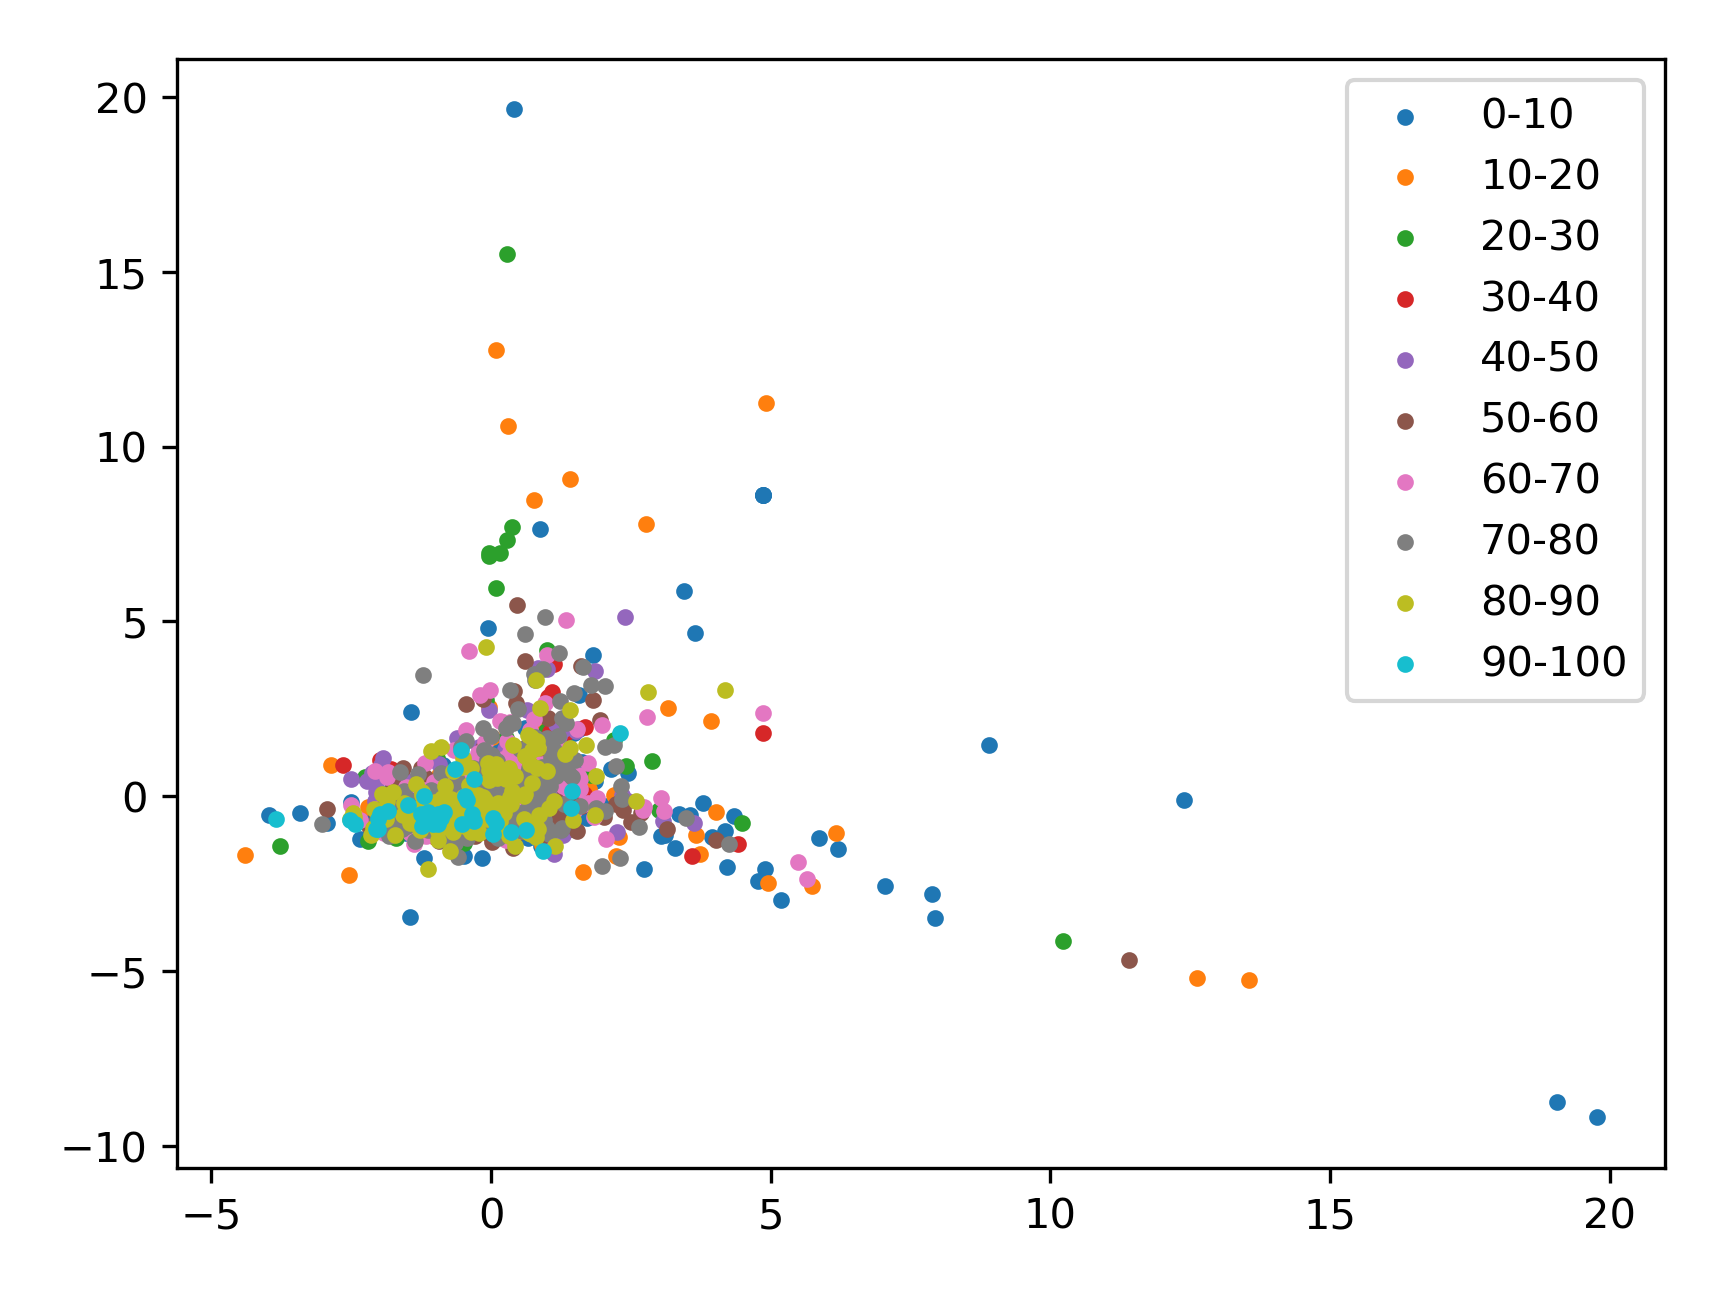
\includegraphics[width=0.75\textwidth]{imgs/visualization_pca.png}
    \caption{Visualization of user embedding vector}
    \label{fig:user_embedding_visualization}
\end{figure}

We can see that points corresponding to the most active groups (80-100) are centered near the origin, while points for the less active groups are distributed along two nearly orthogonal directions. This provides an intuitive explanation for our observations: data from groups 80-100 can boost the overall performance of most users because they roughly lie in the center of most points; but aggregating data across the less active users (0-80) degrades their own performance, because such users are extremely heterogeneous and distinct from each other.

% \section{Additional Discussions about Experiments}
% In this section we provide more details about the experiments in Section \ref{sec:exp}. Our code for conducting these experiments is provided in the supplementary. The experiments involving various threshold values (logarithmically spaced between $10^{-2}$ and $10^{3}$) were split to run on 16 machines, each with a 10-core Xeon processor and 256 GB memory.

% % \textbf{Pre-processing steps of the real-world datasets}:
% \subsection{Pre-processing Steps of the Real-world Datasets}
% The three real-world datasets used in our experiment, i.e., LastFM, Delicious and MovieLens, are public recommendation datasets. Specifically, the LastFM dataset was extracted from the music streaming service Last.fm, and the Delicious dataset was extracted from the social bookmark sharing service Delicious. They were made availalbe by the HetRec 2011 workshop. The LastFM dataset contains $N=1892$ users, 17632 items (artists), and $T=96733$ interactions. We consider the ``\textit{listened artists}'' in each user as positive feedback. The Delicious dataset contains $N=1861$ users, 69226 items (URLs), and $T=104799$ interactions. We treat the bookmarked URLs in each user as positive feedback. 
% The MovieLens dataset used in the experiment is extracted from the MovieLens 20M dataset by keeping users with over $3000$ observations, which results in a dataset with $N=54$ users, 26567 items (movies), and $T=214729$ interactions.
% % that contains 20 million ratings with 27,000 movies and 138,000 users.
% % the MovieLens 20M dataset by keeping users with denser observations, which results in 54 users and 26567 items (movies).
% We consider all items with non-zero ratings as positive feedback in this dataset.
% On the LastFM and Delicious datasets, we extracted TF-IDF feature vectors using tags associated with each item; and on the MovieLens dataset, we also used information from items' metadata, such as movie titles, genres, etc., in addition to the tags, to construct the context vector. We then applied PCA to the resulting TF-IDF feature vectors, and retained the first 25 principle components as the context vectors, i.e., $d=25$. Then we normalized all features to have a zero mean and unit variance in each dimension. To generate the interaction sequence for each user, at each time step when a particular user $i_{t}$ is served, the candidate arm pool for user $i_{t}$ is generated by keeping the item with positive feedback at this time step and sampling another 24 unrated/non-interacted items from this user, i.e., $K=25$.

% \subsection{Discussions about Experiment Results}
% We discuss the experiment results given in Figure \ref{fig:a}-\ref{fig:f}. Note that in the scatter plots (Figure \ref{fig:a}, \ref{fig:b}, \ref{fig:d}, \ref{fig:e}, \ref{fig:f}), 
% % the x-axis is the total communication cost at iteration $T$ and the y-axis is the corresponding accumulative regret/reward at iteration $T$. 
% each dot denotes the accumulative communication cost (x-axis) and regret/normalized reward (y-axis) that an algorithm (\modelone{}, \modeltwo{}, or \modelbaseline{}) with certain threshold value (labeled next to the dot) has obtained at iteration $T$. For example, in the line plot in Figure \ref{fig:sim_hetero_linePlot} that shows more details about how regret and communication cost change over the course of federated bandit learning, the final results of the four algorithms at iteration $T=30000$ in Figure \ref{fig:sim_hetero_linePlot} are used to plot four dots in Figure \ref{fig:b}. 
% % These scatter plots offer a more thorough view of how well the algorithms balance regret/reward and communication cost.

% \begin{figure}[h]
% % \vspace{-2mm}
% \centering
% 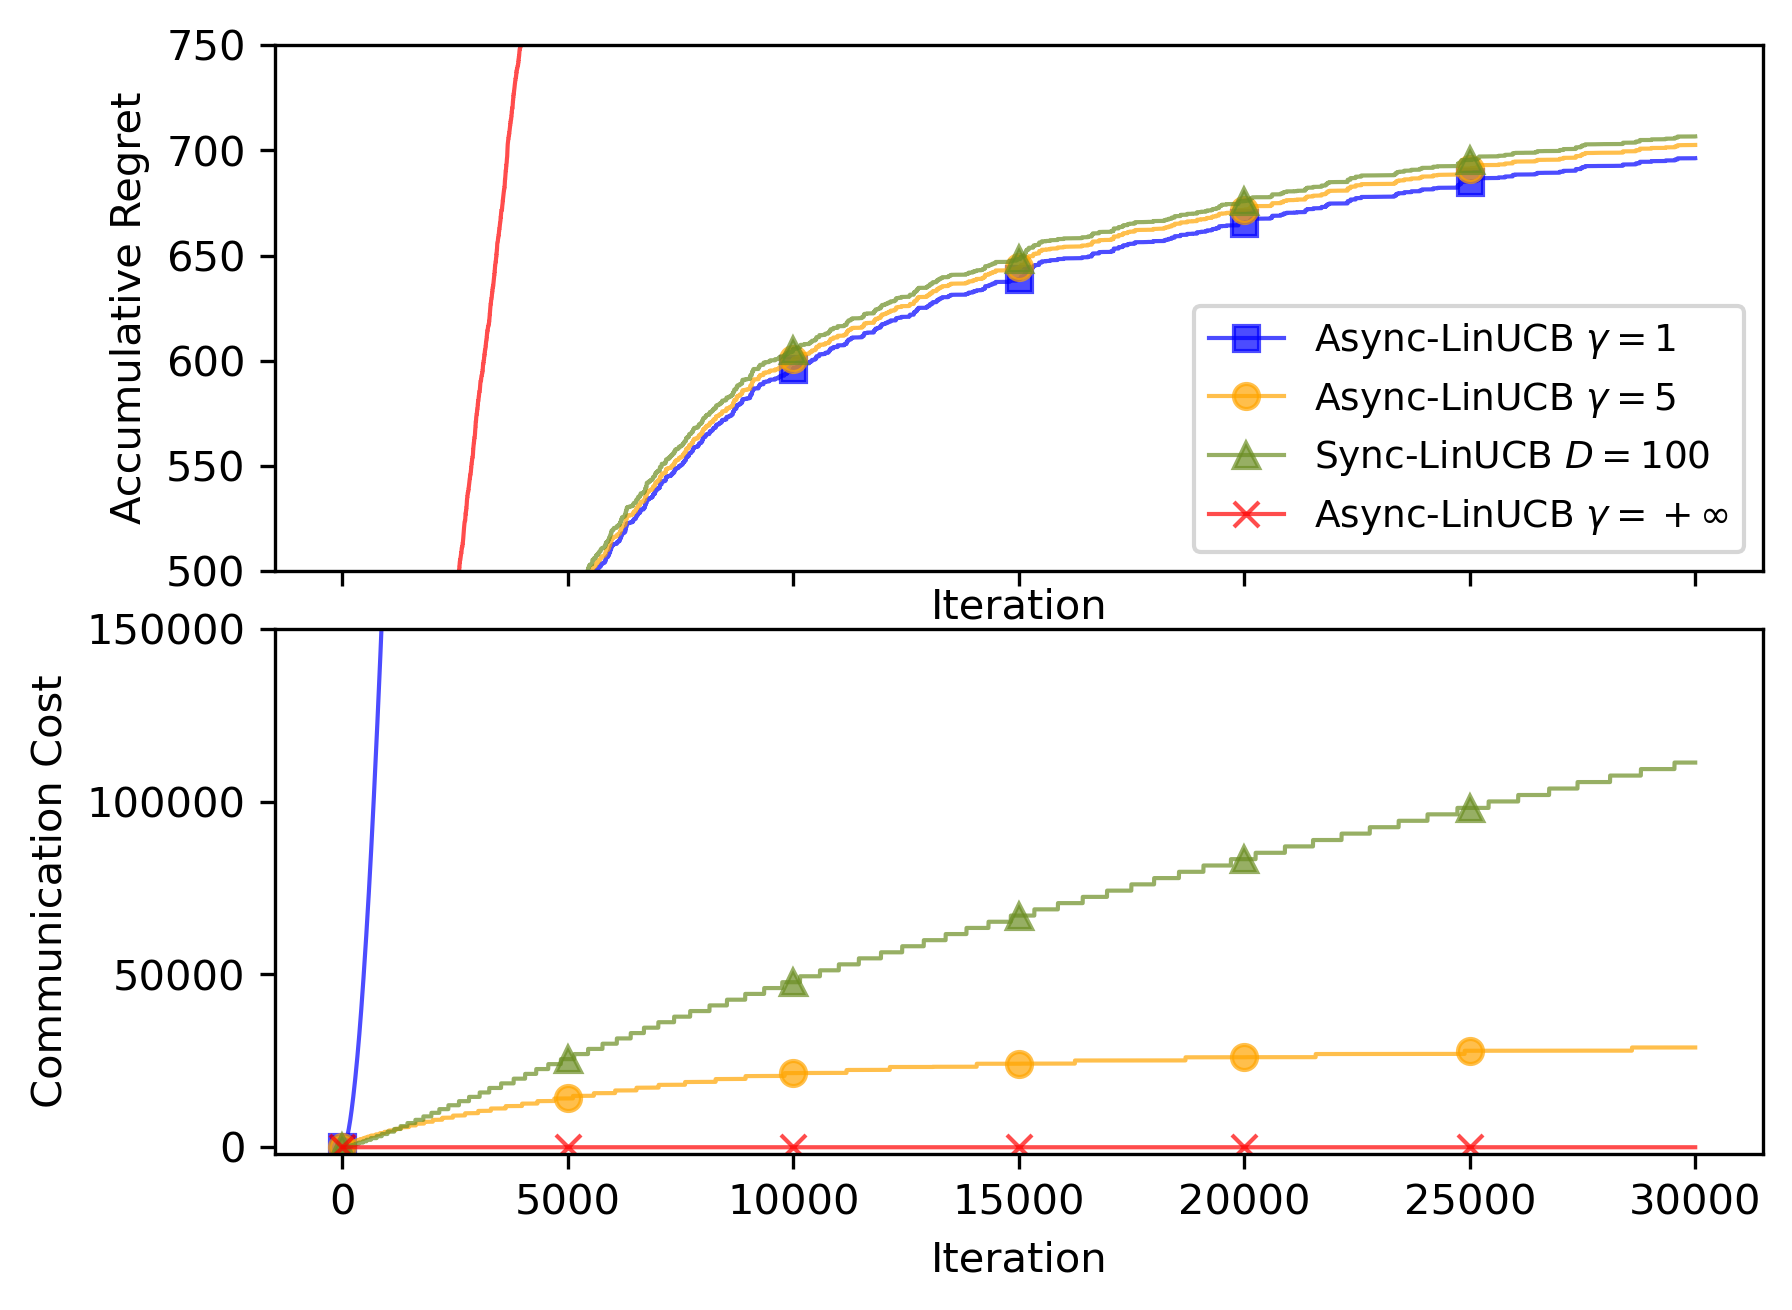
\includegraphics[width=0.65\linewidth]{imgs/sim_hetero_30000_supplementary.png}
% \caption{Results on synthetic dataset: homogeneous clients with non-uniform distribution.}
% \label{fig:sim_hetero_linePlot}
% % \vspace{-3mm}
% \end{figure}

% % \textbf{Results on synthetic datasets}: 
% \subsubsection{Results on synthetic datasets}
% To validate our theoretical analysis in Section \ref{subsec:async_LinUCB} and Section \ref{subsec:async_LinUCB_AM}, two sets of simulation experiments were conducted.
% First, the purpose of simulation experiment in homogeneous client setting is to
% % compare how well the algorithms can balance regret $R_{T}$ and communication cost $C_{T}$ under uniform and non-uniform client distributions, as well as 
% validate our theoretical comparison between \modelone{} and \modelbaseline{} (see Section \ref{subsec:async_LinUCB} and Section \ref{sec:tb_theretical}), i.e., how well the algorithms balance regret $R_{T}$ and communication cost $C_{T}$ under uniform and non-uniform client distributions. Second, the purpose of simulation experiment in heterogeneous setting is to validate our regret upper bound for \modeltwo{} (see Section \ref{subsec:async_LinUCB_AM}), i.e., how the portion of shared components $\frac{d_{g}}{d_{g}+d_{i}}$ affects the regret of \modeltwo{}.

% (1) Homogeneous clients (Figure \ref{fig:a}-\ref{fig:b}): 
% From both Figure \ref{fig:a} and Figure \ref{fig:b}, we can see that the use of event-triggered communication significantly reduces $C_{T}$ while attaining low $R_{T}$, compared with synchronizing all the clients at each time step (\modelone{} with $\gamma=1$). In Figure \ref{fig:a}, \modelbaseline{} has lower $C_{T}$ than \modelone{} under the same $R_{T}$, and in Figure \ref{fig:b}, \modelone{} has lower $C_{T}$ than \modelbaseline{} under the same $R_{T}$, which conform with our theoretical results (see Table \ref{tb:theoretical_comparison}).
% % Among all the algorithms compared, \modelone{} with $\gamma=5$ and $\gamma=8$ and \modelbaseline{} with $D=\frac{T}{d \log{T}}$ strike a good balance between regret and communication cost. The other algorithms either incur a very high regret, i.e. \modelone{} with $\gamma=+\infty$ (as no communication can be triggered), or incur too much communication cost, i.e., \modelone{} with $\gamma=1$ and \modelbaseline{} with $D=\frac{T}{d N \log{T}}$ (as they always communicate). And almost in all results, both synthetic and real-world datasets, always communicating (i.e., \modelone{} with $\gamma=1$) costs significant overhead in communication, while it does not necessarily lead to an obvious advantage in regret. This suggests the necessity and benefit of our event-triggered communication control. In addition, the results for \modelbaseline{} with $D=\frac{T}{d N \log{T}}$ and $D=\frac{T}{d \log{T}}$ conform with our theoretical analysis in Remark \ref{rmk:regret_comm}, e.g., it incurs higher regret when matching the communication cost with \modelone{} or higher communication cost when matching the regret with \modelone{}. 
% % \modelone{} with $\gamma=1$ and \modelbaseline{} with $D=\frac{T}{d N \log{T}}$ attain the lowest regret, but also incur much higher communication costs compared with other algorithms.

% (2) Heterogeneous clients (Figure \ref{fig:c}): By increasing the portion of shared components $\theta^{g}$ in the bandit parameter, we can observe a clear trend in both regret and communication cost, i.e., the regret keeps decreasing while the communication cost keeps increasing. This validates our theoretical analysis about $R_{T}$ and $C_{T}$ in Section \ref{subsec:async_LinUCB_AM}. With $d_{g}$ increases and $d_{l}$ decreases, the first term in the upper bound of $R_{T}$ dominates (which grows slower w.r.t. $N$ compared with the second term), leading to the decreased regret, but the communication cost would increase since $C_{T}=O(d_{g} N \log{T})$.

% \subsubsection{Results on real-world datasets}
% % \textbf{Results on real-world datasets}:
% From the experiments on synthetic dataset, we have validated our upper bounds on the regret and communication cost of \modelone{} and \modeltwo{}. 
% %However, we should note that our theoretical results are based on a slightly stronger assumption on the context vectors (see Assumption \ref{assump:context_diversity}), compared with \modelbaseline{}. 
% %Therefore, we want to validate whether such an assumption is reasonable in practice, i.e., whether our algorithms can still work properly on the real-world datasets that contain TF-IDF feature vectors extracted from the tags and metadata of the items. 
% We continue investigating the effectiveness of our proposed solution on real-world datasets. In addition, since these real-world datasets do not necessarily satisfy the assumption that all the clients are homogeneous, in other words not all the users have the same preference, we pay special attention to \modeltwo{} in the comparison, by setting $x_{g} \equiv x_{i}, \forall i \in [N]$, as mentioned in Section \ref{subsec:problem_formulation}. This allows the clients to learn a global model collaboratively, and in the meantime each learns a personalized model independently. Intuitively, this should make \modeltwo{} more robust to different settings, i.e., the clients are either homogeneous or heterogeneous.

% %First, from the results on all three datasets (Figure \ref{fig:d}-\ref{fig:f}), the performance of \modelone{} is as good as that of \modelbaseline{}, which indicates Assumption \ref{assump:context_diversity} is still reasonable with the TF-IDF feature vectors. Especially in the results on MovieLens dataset (Figure \ref{fig:f}), whose data conforms with our homogeneous clients assumption as we will see below, we can see the dots corresponding to \modelone{} and \modelbaseline{} have very similar patterns as that in the ideal simulation environment (Figure \ref{fig:a}).

% To understand the results of these algorithms on the three real-world datasets, we can first look at how well the two extreme cases, \modelone{} with $\gamma=1$ and \modelone{} with $\gamma=+\infty$ perform. 

% (1) LastFM \& Delicious (Figure \ref{fig:d}-\ref{fig:e}): 
% On both LastFM and Delicious datasets, \modelone{} with $\gamma=+\infty$ (illustrated as the red dot) attains very high reward, which suggests users in these two datasets have very diverse preferences, such that aggregating their data has a negative impact on the performance. 
% Since the homogeneous clients assumption does not hold in this case, both \modelone{} and \modelbaseline{} perform as badly as the extreme case of \modelone{} with $\gamma=1$, which is especially true when the clients frequently communicate with each other, i.e., with lower threshold values.
% % , and the more the clients communicate with each other, the lower rewards they will obtain, due to the mistakenly aggregated heterogeneous data. 
% In comparison, \modeltwo{} attains relatively good performance even when the clients frequently communicate with each other, as it allows personalized models to be learned on each client.

% (2) MovieLens (Figure \ref{fig:f}): 
% Note that on this dataset, \modelone{} with $\gamma=1$ attains very high reward, which indicates that the users share similar preferences, so that data aggregation over different users becomes vital for good performance. 
% In this case, learning a personalized model on each client becomes unnecessary and slows down the convergence of model estimation, which leads to the lower accumulative reward of \modeltwo{} compared with the other two algorithms.
% % And as \modeltwo{} requires each client to learn a personalized model, which becomes unnecessary in this case, 
% % it slows down convergence of the model estimation and thus leads a lower reward compared with the other two algorithms.
% However, we can see that \modeltwo{} can still benefit from collaborative model estimation, as it has a much higher accumulative reward than the extreme case of \modelone{} with $\gamma=+\infty$.

% % (1) LastFM \& Delicious (Figure \ref{fig:d}-\ref{fig:e}): 
% % On both LastFM and Delicious datasets, disabling any communication and running LinUCB on each client independently (\modelone{} with $\gamma=\infty$, which is illustrated as the red dot) attains fairly high reward, particularly when compared with synchronizing all the clients in each time step (\modelone{} with $\gamma=1$). This suggests users in these two datasets have very diverse preferences, such that directly aggregating all their data has a negative impact on the performance. 
% % In Figure \ref{fig:d}, \modeltwo{} performs much better than \modelone{} and \modelbaseline{} under all $C_{T}$, which indicates the users' bandit parameters in LastFM are diverse but very likely to have a common center, such that this multi-task formulation by \modeltwo{} has a clear advantage.
% % In Figure \ref{fig:e}, \modelone{} with high thresholds performed the best. Our hypothesis is that the most active users in Delicious share similar parameters, while the less active users have more diverse parameters. Therefore, setting a high threshold for \modelone{} essentially blocks the upload communications from the less active clients, but allows the most active clients to collaborate in model estimation, which explains its higher accumulative reward compared with other algorithms. In comparison, the global synchronization step of \modelbaseline{} asks all the clients to upload their data, which introduces distortion to model estimation due to the mistakenly aggregated heterogeneous data.

% % On both LastFM and Delicious datasets, \modelone{} with $\gamma=\infty$ performs fairly well in terms of regret, despite it disables any communication among the clients. It suggests users in these two datasets may be very diverse in their preferences. As a result, the homogeneous clients assumption might not be true on these two datasets, which also explains the inferior performance of \modelone{} with $\gamma \in \{1,2,5,8\}$ and \modelbaseline{}. In comparison, we can find that \modeltwo{} performs well on these two datasets, as it supports personalized model learning in each user. This result shows the effectiveness of \modeltwo{} in addressing ``\emph{non-IIDness}" in individual users' observations.

% % (2) MovieLens (Figure \ref{fig:f}): 
% % Note that for MovieLens dataset, synchronizing all the clients in each time step (\modelone{} with $\gamma=1$) attains very high reward, which indicates that users in the MovieLens dataset share similar parameters, so that data aggregation over different users becomes vital for good performance. Since this dataset conforms with our assumption of homogeneous clients (Section \ref{subsec:problem_formulation}), we can see the dots corresponding to \modelone{} and \modelbaseline{} have very similar patterns as that in Figure \ref{fig:a}. And as \modeltwo{} requires each client to learn personalized components, which is unnecessary in this setting, it has a lower reward compared with the other two algorithms.

% % Note that on MovieLens dataset, \modelone{} with $\gamma=1$ and $\gamma=5$, and \modelbaseline{} with $D=\frac{T}{d N \log{T}}$ outperform others, which indicates that users in the MovieLens dataset share much interests in common, so that data aggregation over different users becomes vital for the performance. In addition, compared to \modelone{} with $\gamma=1$ that synchronizes the clients in each round, \modelone{} with $\gamma=5$, and \modelbaseline{} with $D=\frac{T}{d N \log{T}}$ are much more communication efficient, which shows the effectiveness of event-triggered communication. We should also note that on MovieLens dataset \modeltwo{} obtains similar rewards as \modelone{} with $\gamma=+\infty$. This is because when \modeltwo{} is applied to homogeneous clients, it would incur the additional term of regret (as discussed in Section \ref{subsec:async_LinUCB_AM}) due to the independently learnt local components, which matches that of running $N$ independent LinUCB algorithms for each client.
